\chapter{Resonance Searching Strategy}
The diboson physics was well-understood in 20th century with the experiments hosted by Large Electron Positron Colliders (LEP), and it also plays an important role as the portal to many BSM models. For the direct search of new physics in diboson ``medium'' states in this thesis, it is aiming for the mass resonance of new particles which could be from Extended Gauge Model, Extra Dimensions or Technicolor models.
\\
\\In the study here, $WW$ and $WZ$ are the two medium states of interest through the production of gluon-gluon fusion, Drell-Yan process, or vector boson fusion. The vector boson fusion is the fusion process of two vector bosons ($W$ or $Z$) emitted from two incoming quarks, and the two quarks are then scattered into two energetic jets with wide $\eta$ separation and high invariant mass. The production processes could be seen in Fig. \ref{Fig:Xprod} as Feynman diagrams. For the final state, one $W$ boson would decay leptonically ($W\rightarrow l\nu$) into an electron or muons accompanied by a neutrino with the corresponding flavour, while the decay of $tau$ is not considered here. For the other boson, $W$ or $Z$,  it is supposed to decays hadronically into two quarks reconstructed into two $R=0.4$ jets or one $R=1.0$ jet. ($W/Z\rightarrow jj$ or $W/Z\rightarrow J$). The benefit of choosing this final state is to have the high branch ratio from the hadronic decay and suppress the QCD contamination by the leptonic side. This study is conducted in a wide range of candidate particle mass ranging from $300GeV$ to $5TeV$. If the mass of a resonance particle is high enough ($m>\tilde1~TeV$), the outcoming two quarks in the final state would be highly boosted. In the scenario, their reconstruction could not be resolved as two jets with $R=0.4$, so a larger cone of $R=1.0$ is applied to collect their signatures into a single fat jet. 
\\
\\This search was conducted with the $36.1fb_{-1}$ data collected by the ATLAS detector in 2015 and 2016 with pp collisions at $\sqrt{s}=13TeV$. 

\begin{figure}[htp]
	\centering
	\subfloat[Drell-Yan Process]{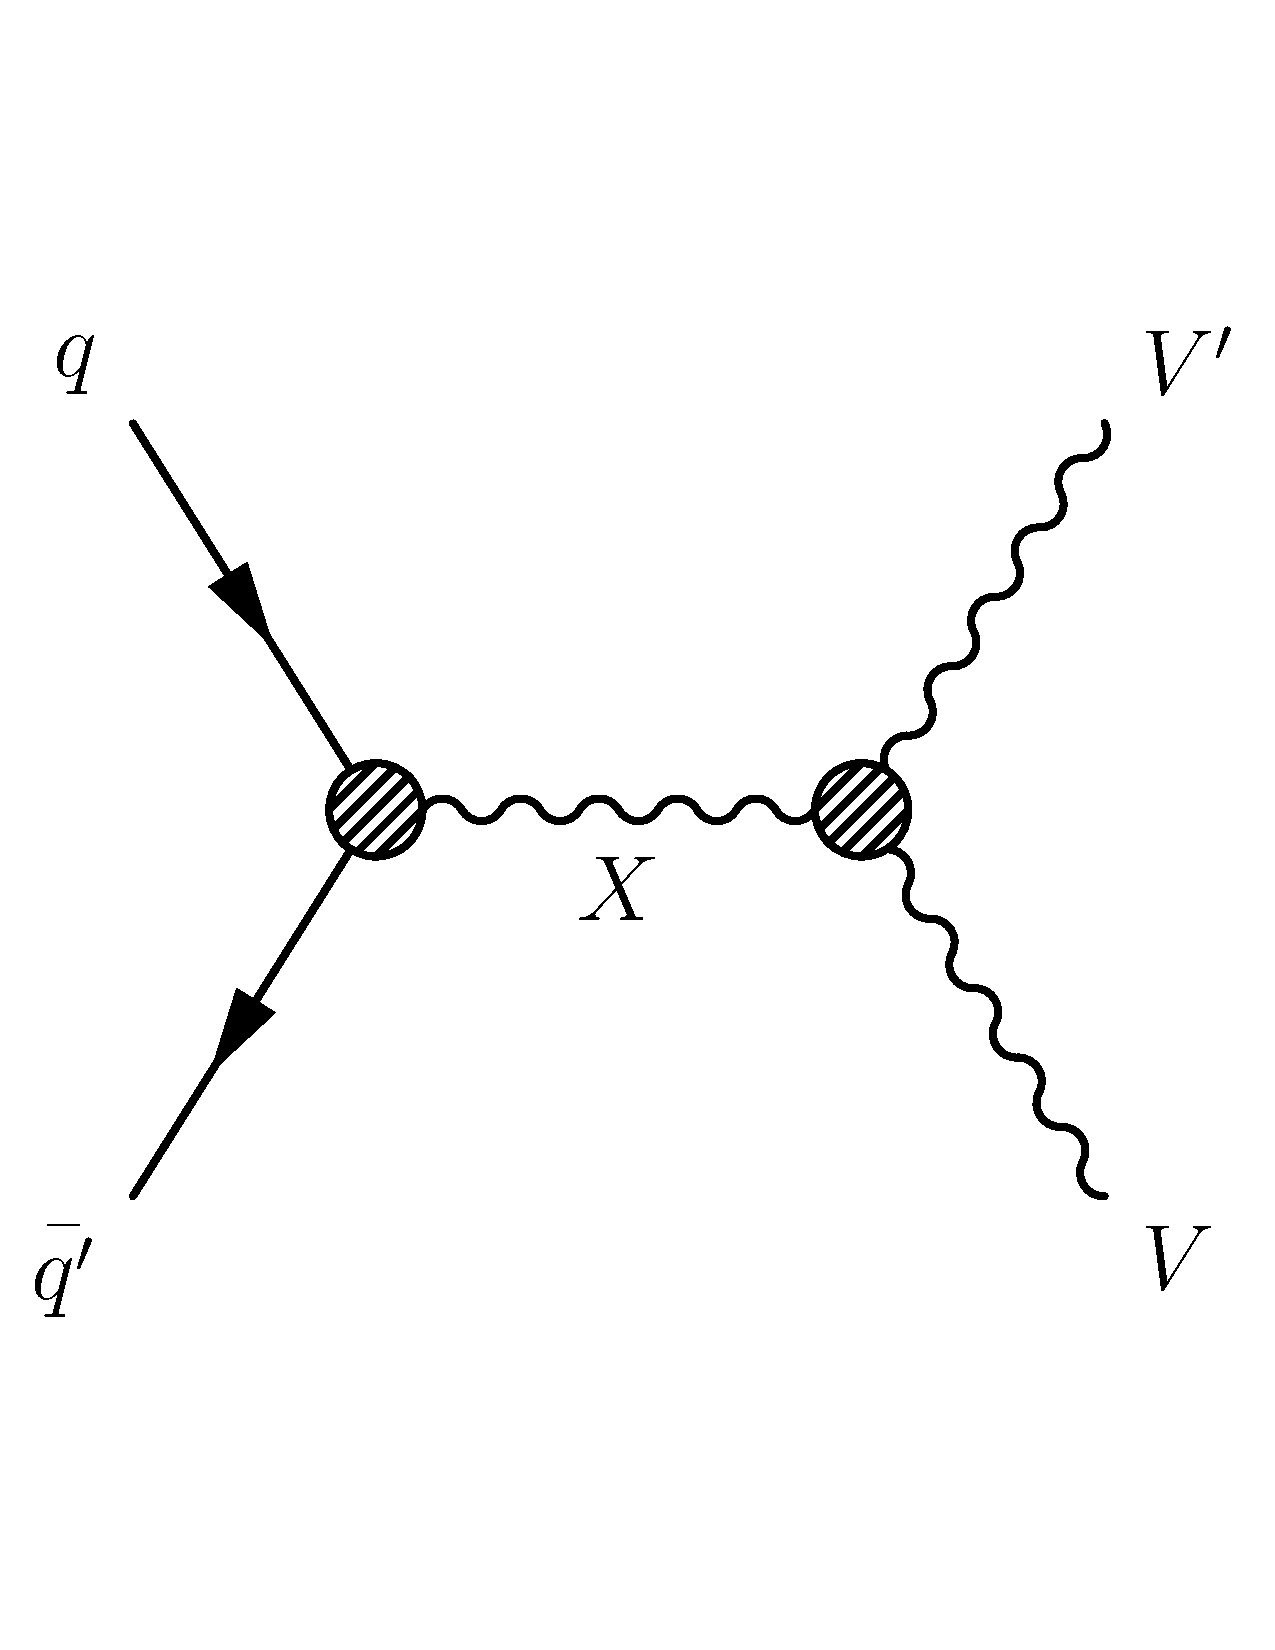
\includegraphics[width=.3\textwidth]{Chapter3/DY_X.pdf}}\hfill
	\subfloat[gluon-gluon Fusion]{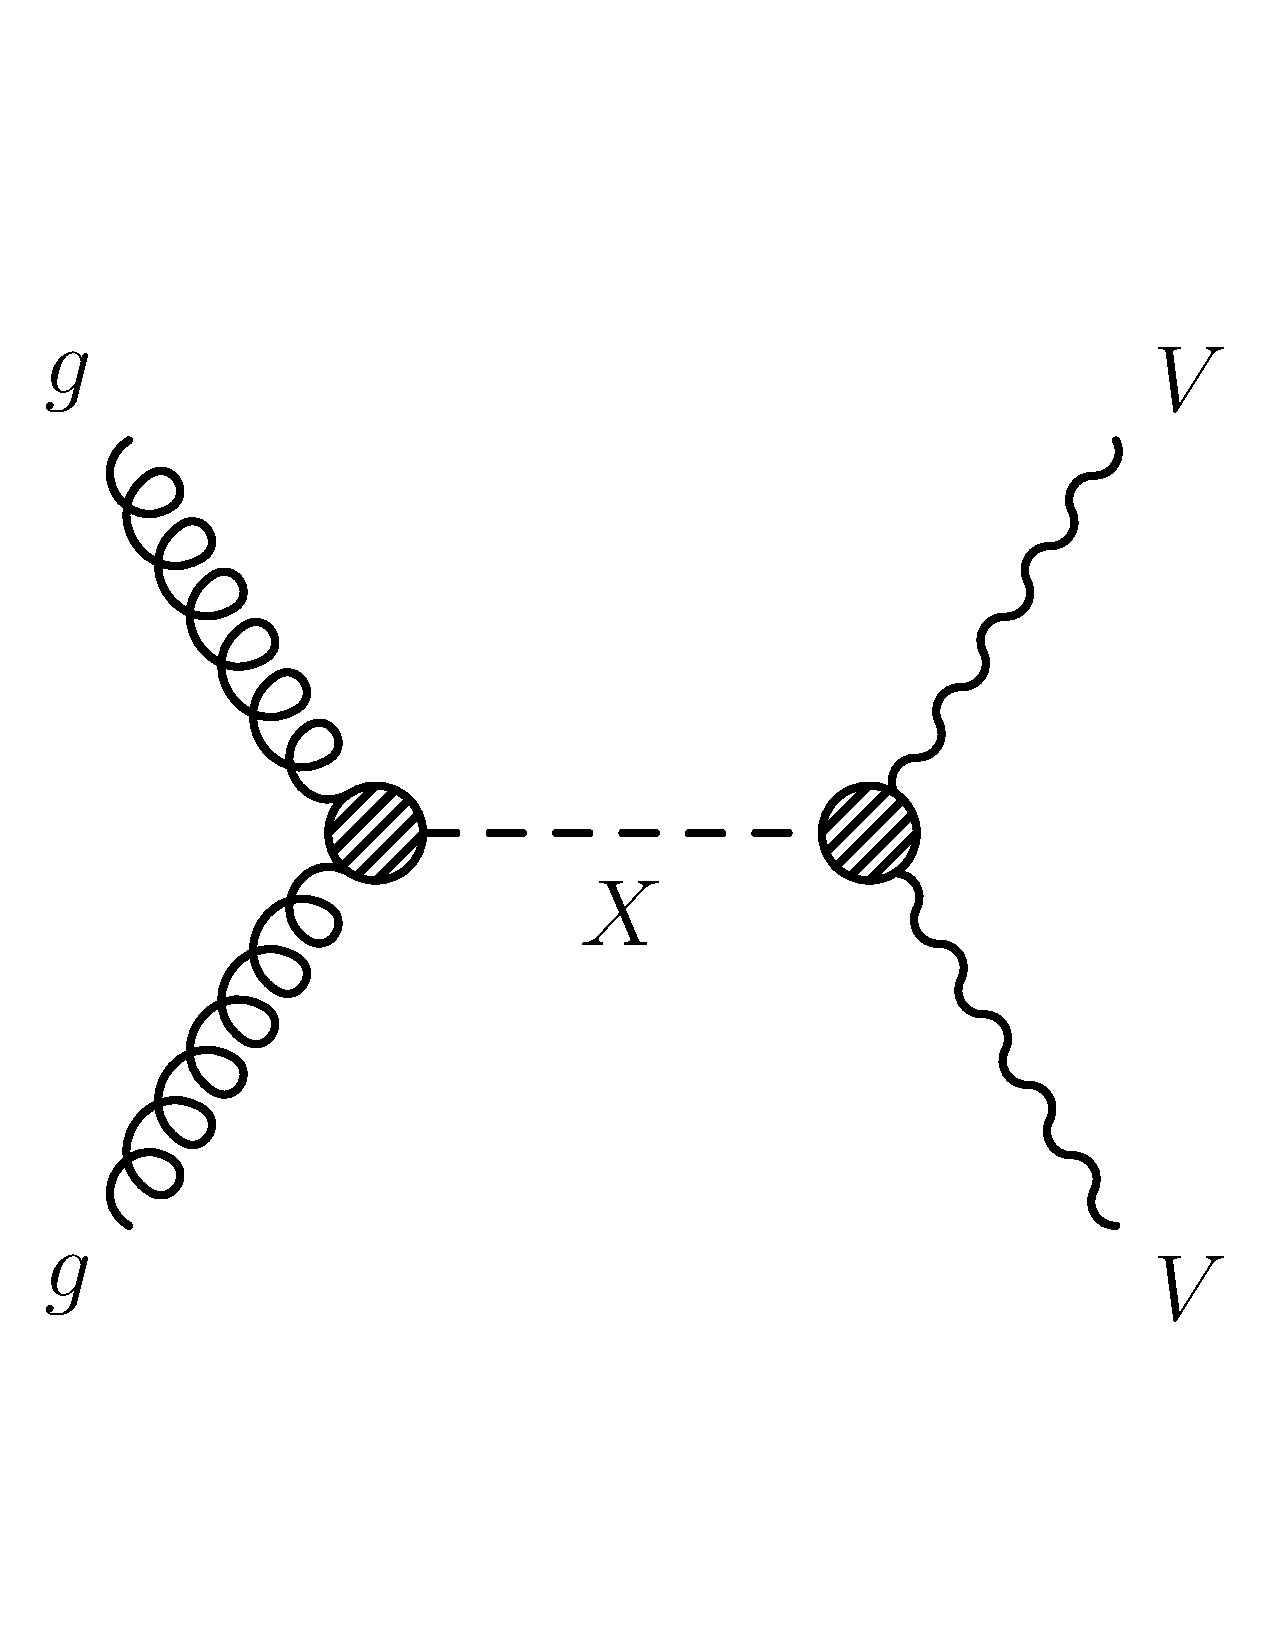
\includegraphics[width=.3\textwidth]{Chapter3/ggF_X.pdf}}\hfill
	\subfloat[Vector Boson Fusion]{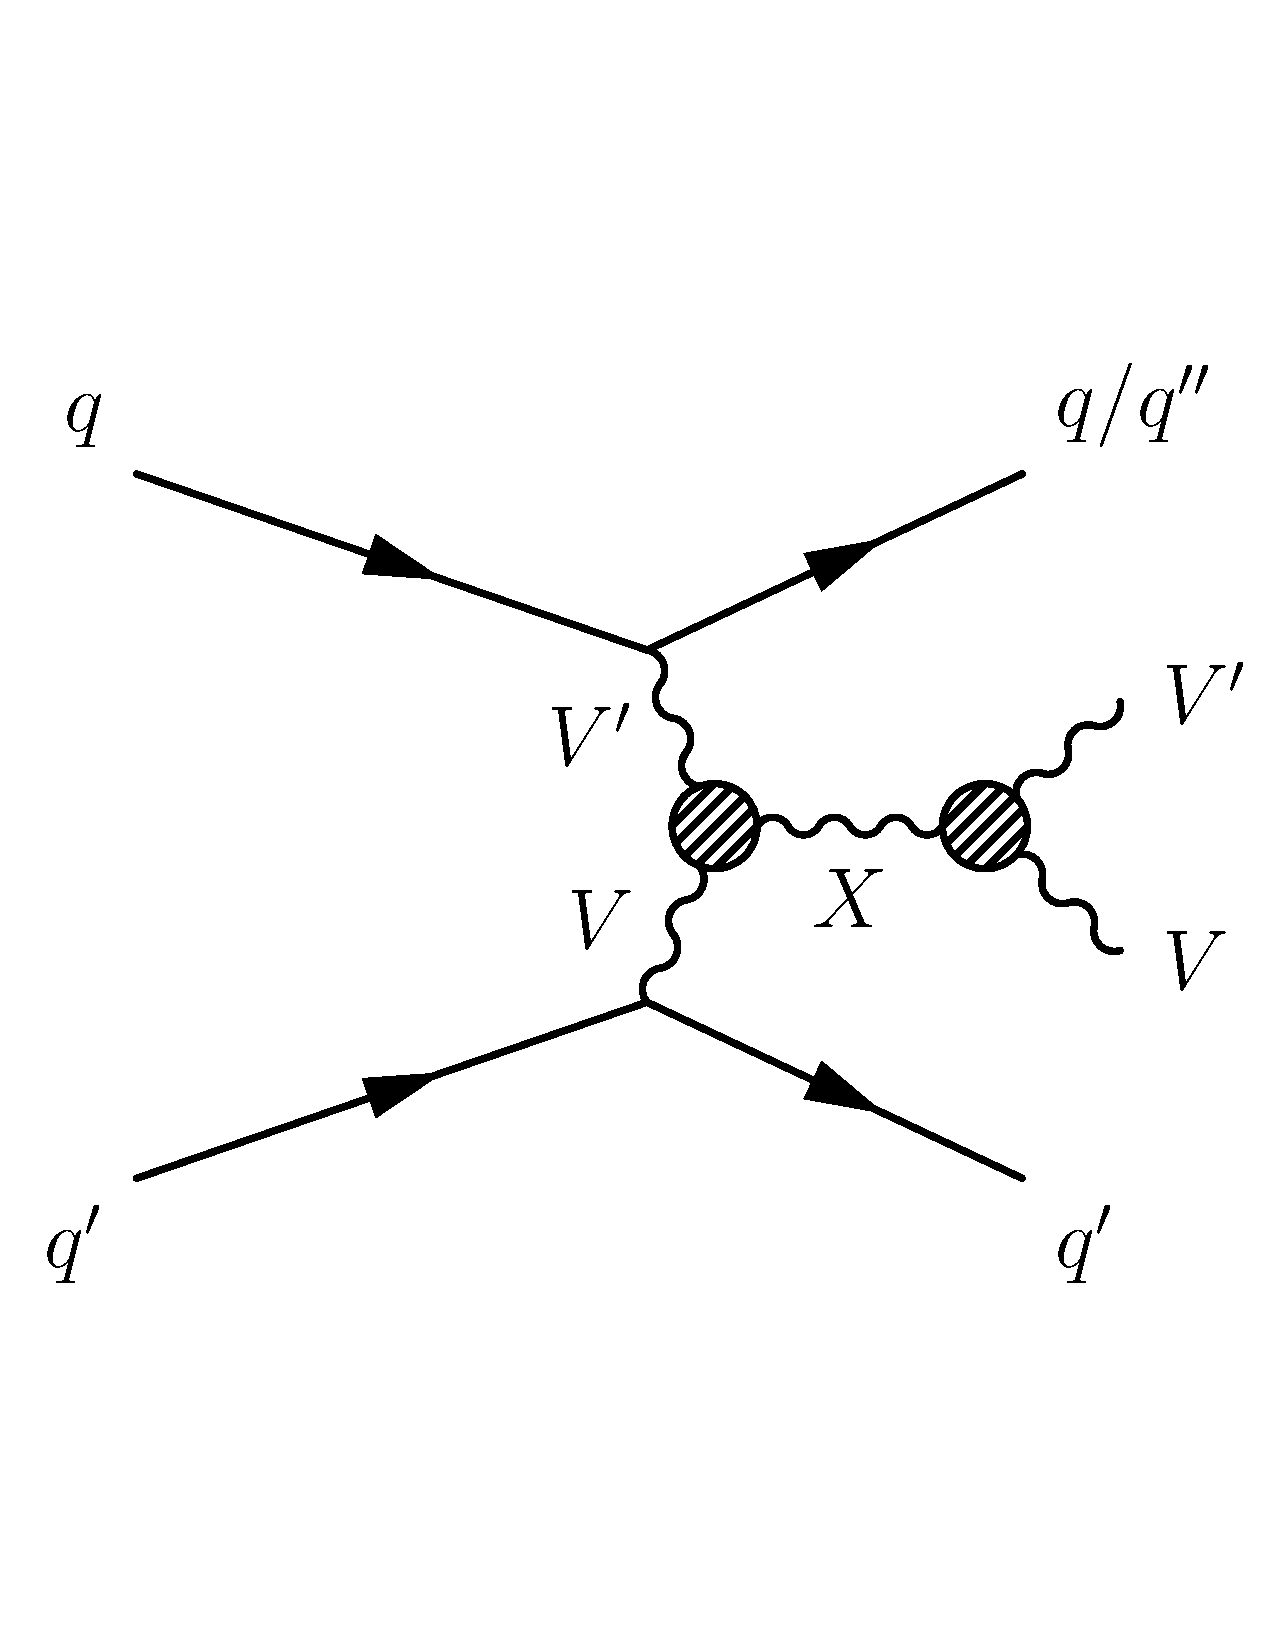
\includegraphics[width=.3\textwidth]{Chapter3/VBF_X.pdf}}
	\caption{The Feynman diagrams of different production mechanisms for particle X which decays into two SM bosons.}
	\label{Fig:Xprod}
\end{figure}
\section{Signal Models}
\label{sec:signal_intro}
In SM, bosons are the force carrier and also maintain the conservation of certain physical quantities which are called symmetry. To seek for the solution of unsolved problems in SM, many new models are predicting the existence of new bosons corresponding to unknown interactions or symmetries, and they also have strong coupling to the SM bosons which provide the access to verify those theories. However, the existing new models are constructed with many free parameters, and each set of them needs a dedicated analysis from experiment side, which is impossible in reality. Therefore, a simplified model with only the kinematic parameters related to resonance mass is introduced for which experiment could provide the precise measurement to on-shell bosons.  
\\
\\This strategy could scan through many models, so it is defined as a general search. However, to give better separation between signal and background, three benchmarks are applied in this analysis for sensitivity optimization which corresponds to bosons with different spins: $spin=0$, narrow width approximation Higgs boson (NWA); $spin=1$ heavy vector triplet (HVT); $spin=2$, Randall–Sundrum model graviton (RSG).
\\
\\{\bf Narrow Width Approximation Higgs Boson}
\\
\\With the problem in Higgs boson naturalness, some extended models predict the existence for the Higgs bosons with even higher mass to complete SM. The simplest scenario is the addition of one scalar singlet into the SM Lagrange Higgs sector providing the generic framework to analyse scaler singlets in LHC signatures. This will extend the potential in Eq. \ref{Eq:sm_higgs_potential} to:
\begin{equation}
 \begin{aligned}
    V(\Phi)={} & \mu^2|\Phi^\dagger\Phi|+\lambda(|\Phi^\dagger\Phi|)^2+\frac{\delta_1}{2}\Phi^{\dagger}\Phi S \\
   & +\frac{\delta_2}{2}\Phi^{\dagger}\Phi S^2+(\frac{4\delta_{1}\mu^2}{\lambda})S+\frac{\kappa_2}{2}S^{2}+\frac{\kappa_3}{3}S^{3}+\frac{\kappa_4}{4}S^{4}
 \end{aligned}
\end{equation}
The first two terms are still the same to SM, but the following ones are with the new scalar singlet, $S$.  The couplings between the SM Higgs field and the addition scalar singlet are $\delta_1$ and $\delta_2$, which are chosen for the mixing between them. The last four linear terms is to eliminate the vev contribution from $S$. With this extension, two Higgs bosons arise from this formula: $H_1$ and $H_2$
, and the corresponding mass matrix could be shown as:
\begin{equation}
M_{H}^2 = \left[ \begin{array}{l r} 2\lambda \nu^2 &  \delta_1 \nu \\ \delta_1 \nu& \frac{\lambda_{s}\nu^2}{2} \end{array} \right]
\end{equation}
with $\lambda_s = \delta_2+2\frac{\kappa_2}{\nu^2}$ and $\nu$ as vev of $246GeV$. After proper rotation, the Higgs bosons related to the SM Higgs field and the scalar singlet are presented as:
\begin{equation}
 \left[ \begin{array}{c} H_{1} \\ H_{2} \end{array} \right] = \left[ \begin{array}{l r} \cos{\phi} & \sin{\phi} \\ -\sin{\phi}& \cos{\phi} \end{array} \right] \left[ \begin{array}{c} \Phi \\ S \end{array} \right]
\end{equation}
where $\phi$ is the mixing angle. With the two formula, the mass eiganstate could be given as:
\begin{equation}
M_{H1,H2} = \frac{4\lambda+\lambda_{S}}{4}\mp\frac{\sqrt{\nu^4(4\lambda-\lambda_{S})^2+4\nu^2\delta_1^2}}{4}
\end{equation}
with the solution to $\phi$ as:
\begin{equation}
\tan{\phi} = \frac{4\delta_1}{\nu(4\lambda-\lambda_{S})-\sqrt{\nu^2(4\lambda-\lambda_{S})^2+4\delta_1}}
\end{equation}
With the discovery of SM Higgs boson ($H_{1}$), the mixing angle $\phi$ between $\Phi$ and $S$ is supposed to be small, and $H_2$ is almost exactly the scalar singlet boson. With the condition of $\mathbb{Z}_2$ is slightly broken for $\delta_1$ and $\kappa_3$ approximating to 0, it would make the decay width of $H_2$ relatively small. To simplify the analysis, ``narrow width approximation'' is applied assuming $\Gamma_{H_2}<<m_{H_2}$, so this particle only decays at the mass pole.
\\
\\{\bf Heavy Vector Triplet}
\\
\\Heavy vector bosons are predicted by many new BSM theories with the coupling to quarks, leptons, SM vector bosons and Higgs boson, which constructs a wide phase space. To examine the suitable theories, this study attempts to investigate all the couplings with the set-up of one neutral heavy boson $Z'$ and two degenerate charged bosons, $W'^{\pm}$ with the given coupling constant, $g_{V}$. For optimization,  two models are taken as the benchmarks. Model A with an additional symmetry breaking to SM, $SU_{1}(2)\times SU_{2}(2) \times U(1) \rightarrow SU_{L}(2) \times U(1)$ giving a weak coupling: $g_{V} \sim \mathcal{O}(1)$. For the scenario of strong coupling (new bosons have stronger couplings to fermions), Minimal Composite Higgs Model is taken as model B with the symmetry breaking, $SO(5) \rightarrow SO(4)$ for $4\pi \geq g_{V} \geq 1$. However, because the decay width is proportional to the coupling constant, and the focus of this search is for the narrow resonance, only $6 \geq g_{V} \geq 1$ is considered with $\Gamma_{V}/m_{V}$ below $10\%$.
\\
\\To simplify the models, the coupling strengths to all fermions are set equal with scale of $g^2c_{F}/g_{V}$ where $g$ is the $SU_{L}(2)$ gauge coupling, and $c_{F}$ is the dimensionless coefficient between bosons and fermions set as a free parameters of order one in the phase space of interest. As the coupling scale is proportional to $1/g_{V}$, model A turns to be more sensitive to the fermionic production with Drell-Yan process, while model B is well-suppressed. In the contrary, the coupling to bosons is governed by $c_{H}g_{V}$ with $c_{H}$ as the universal coupling among bosons. Therefore, model B has better sensitivity for higher branch ratio of the decay channel of diboson in this analysis than model A. For the interpretation, the two parameters, $g^2c_{F}/g_{V}$ as well as $c_{H}g_{V}$, construct a two-dimension phase space, and with the varied sensitivity, all the regions could be explored with production rate and decay branch ratio. 
\\
\\As the coupling to all bosons are the same ($c_{H}g_{V}$), the neutral and charged heavy boson ($Z'$ and $W'^{\pm}$) have the same decay branch ratio to all SM bosons:
\begin{equation}
BR(Z'\rightarrow ZH) = BR(Z'\rightarrow W^\pm W^\pm) = BR(W'^\pm \rightarrow W^\pm Z) = BR(W'^\pm \rightarrow W^\pm H)
\end{equation}
However, with the small mixing angle (between SM and BSM bosons), the coupling in the transverse component is well suppressed, and the dominant contribution is from longitudinal component. For the same reason, the coupling to neutral dibosons are also so weak that those channels are ignored in this analysis, which is also applicable to $W\gamma$.  For the coupling to $HH$, they are forbidden due to the concern of momentum and angular momentum conservation. 
\\
\\{\bf Randall-Sundrum Graviton}
\\
\\To solve the hierarchy problem, extra dimensions were proposed as one of the solutions. It leads to the result that the the observed Planck scale, $M_{pl}=2\times10^8GeV$, is already reduced due to the existence of extra dimensions from the orginal scale, $M$. The relation between $M_{pl}$ and $M$ is: 
\begin{equation}
\label{Eq:planck_relation}
M_{pl}^{2} = M^{n+2}V_{n}
\end{equation}
where n is the number of dimensions which are not yet observed, and $V$ is the volume constructed from the extra dimensions regardless of the 4-dimension spacetime. Therefore, the visible spacetime is just a manifold under ($4+n$) dimensions.
\\ 
\\Under Randall-Sundrum model, only one more dimension is needed, which hypothesizes that the 5th dimension is constrained with boundary condition of the $\phi$ periodicity ranged between $-\pi$ to $\pi$ called ``warped bulk'' which bridges two 4-dimension manifolds at $\phi=\pi$  and $\phi=0$ ($\phi$ is taken as the 5th coordinate). The ``Hilbert-Einstein''action under the set-up could be presented as:
\begin{equation}
S = S_{gravity} +S_{obs} + S_{hid}
\end{equation}
\begin{equation}
S_{gravity} = \int d^4x \int^{\pi}_{-\phi}d\phi\sqrt{G}\left[-\Lambda +2M^3R\right]
\end{equation}
\begin{equation}
S_{vis(hid)} = \int d^4x\sqrt{-g_{vis(hid)}}\left[\mathcal{L}_{vis(hid)}-V_{vis(hid)}\right]
\end{equation}
with $\Lambda$ as cosmological constant, R as scalar spacetime curvature, and $g$'s are the determinant of metric tensor matrix,  $g_{\mu\nu}$. $V_{vis}$ and $V_{hid}$ are the constant gravitation potential taken out from the Lagrangian vacuum energy for the visible and hidden spacetime. After inserting the terms into Einstein Feild Equation, it leads to the solution for the spacetime description:
\begin{equation}
ds^2=e^{-2\sigma(\phi)}\eta_{\mu\nu}dx^\mu dx^\nu + r_c^2 d\phi^2
\end{equation}
with
\begin{equation}
\sigma(\phi) = kr_c|\phi| \quad k=\sqrt{\frac{-\Lambda}{24M^3}}
\end{equation}
where $\eta$ is the Minkowski metric, and $r_{c}$ is the constant independent of $\phi$ taken as the ``compactification radius'' of the extra dimension on the orbifolding. As a result, the extra dimension only has the dimensional interval, $\pi r_{c}$, at $\phi=\pi$ in the visible spacetime. Taking the space description into Eq. \ref{Eq:planck_relation}, the relation between $r_c$ and $M_{pl}$ could be derived as:
\begin{equation}
M_{pl}^2=\frac{M^3}{k}\left[1-e^{-2kr_{c}\pi}\right]
\end{equation}
This expression indicates that $M_{pl}$ depends on $kr_{c}$, and the weak gravity could be explained with proper choice of $r_c$. Under the solution, the existence of graviton is then taken as the tensor fluctuation on Minkoski metric: $\eta_{\mu\nu} \rightarrow \eta_{\mu\nu}+\bar{h}_{\mu\nu}(x)$. To estimated its mass, the new spacetime geometry is inserted into the Higgs sector in SM Lagrange , and it gives the result: $m=e^{-kr_{c}\pi}m_{0}$ with $m_{0}$ as the original mass scale in the visible manifold (IR brane), and m as the one in the 5-dimension spacetime. (This relation could also be applied to SM particles.) If $e^{kr_{c}\pi}$ is of order $10^{15}$, the mass scale would be in the scale of $TeV$ under the mechanism which offers the signature verifiable to LHC energy scale with the couplings to SM particles derived from the same way.
\section{Simulation Samples and Derivation}
Each SM background process and mass point of signals are simulated by the procedure mentioned in \ref{sec:simulation}.  To make proper comparison of simulation and data, the event numbers are normalised to theoretical cross section and total data luminosity. However, the modelling of the interactions between the ATLAS detector and particles is not perfect. It leads to the discrepancy in efficiency measurement of different parameters including particle reconstruction, lepton isolation, trigger, or jet b-tagging. To recover this disagreement, a scaling factor is estimated from the comparison between data and MC and applied on the event weight in MC. 
\\
\\Other than the efficiency parameters, the other disagreement comes from the inconsistency in distributions of interaction number per bunching crossing , $\mu$, which is unpredictable in data along the operation period. Therefore, the rescaling called ``pile-up reweighting'' (PRW) is used to modify simulated $\mu$ distribution to agree with data. 
\\
\\After considering all the factors for data-MC comparison, the final simulation event yield could be reweighted to data by:
\begin{equation}
N_{yield} = \mathcal{L}\times XS \times \epsilon_{rec} \times \epsilon_{iso} \times \epsilon_{trigger} \times \epsilon_{b-tagging} \times \epsilon_{prw} / N_{mc}
\end{equation}
where $N_{yeild}$ and $N_{mc}$ are the estimated data and MC event numbers, and $\epsilon$'s stand for the scaling factors of different contributions. 
\\
\\{\bf Background Simulation}
\\
\\Some of the SM processes have the same final state of one lepton, one neutrino and multiple jets to the new physics of interest, so they are called ``irreducible'' background which could not be well-suppressed. This type of backgrounds are estimated from Monte Carlo simulation contributed from W+jets ($W\rightarrow l\nu$), $t\bar{t}$ ($t\rightarrow bW \rightarrow bjj$ and $t\rightarrow bW \rightarrow bl\nu$), diboson ($WW/WZ\rightarrow l\nu jj$), Z+jets ($W\rightarrow l\nu$), and single top.  
\\
\\The events of W/Z+jets are simulated by \textsc{SHERPA} v2.2.1, with the PDF configuration of \textsc{NNPDF30NNLO} as the baseline generator, and the simulation uncertainty is taken by the comparison to other generators detailed in next chapter. With the complicated process of hadronisation including the broad range of jet $p_{T}$ and involved quark flavours, the simulation is done respectively with multiple slices of $max(h_{T}, p_{T}(W/Z))$ ($h_{T}$ is the scalar sum of $p_{T}$ from all jets) and different number of bottom and charm quarks. The involved matrix element for the simulation are up to 2 partons at NLO and 4 partons at LO which is followed by merging into the Sherpa parton shower. The resulting cross section for normalisation is estimated to NNLO of QCD.
\\
\\$t\bar{t}$ events are generated through \textsc{Powheg-Box} v2 with the matrix element calculation provided by \textsc{CT10 PDF} with top quark mass set at $172.5GeV$, and the \textsc{HDAMP} parameters for high $p_{T}$ radiation is set at $1.5m_{t}$. Different from \textsc{SHERPA} as self-contained generator to do parton shower itself, the simulation from \textsc{Powheg-Box} is then interfaced through \textsc{MadSpin} and \textsc{PYTHIA}8.186 tuned by Perugia 2012 (P2012) and \textsc{CTEQ6L1 PDF} sets for spin correlation preservation of top quark decay and the following parton shower, fragmentation and underlying events. The renormalisation and factorisation scale of the whole process are determined by $\sqrt{m_{t}^2+p^2_{T}(t)}$. The $t\bar{t}$ cross section used for normalisation is calculated using \textsc{TOP++} 2.0 with the precision up to NNLO in QCD. To taking in contribution from the soft gluon terms, a re-summation with next-to-next-to-leading logarithmic (NNLL) is applied to make further correction.  
\\
\\Single top events are generated through three different processes: s-, t- and Wt-channel productions (Feynman diagrams are presented in Fig. \ref{Fig:singletop}). For the simulation of Wt and s-channels, the same recipe from $t\bar{t}$ generation is adopted, while the t-channel one is through \textsc{Powheg-Box} v1 with fixed four-flavor CT10f4 PDF set but also followed by the same procedure for decay and parton showering from $t\bar{t}$ generation. The renormalisation and factorisation scales are set respectively for the three channels with:
\begin{itemize}
	\item s-channel $\&$ Wt-channel: $m_{t}$
	\item t-channel 4\times$\sqrt{m_{q}^2+p^2_{T}(q)}$ (q is the quark  associated with the single top quark production)
\end{itemize}
, and the cross section for each production is calculated separately with the description in 
\begin{figure}[htp]
	\centering
	\subfloat[t-channel]{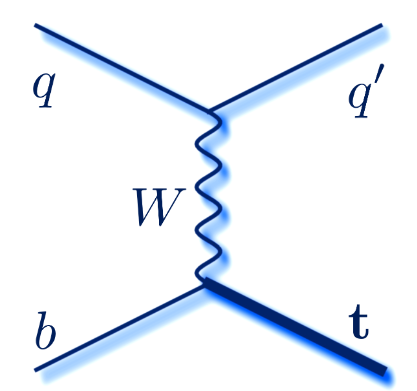
\includegraphics[width=.25\textwidth]{Chapter3/t-channel.png}}\hfill
	\subfloat[Wt-channel]{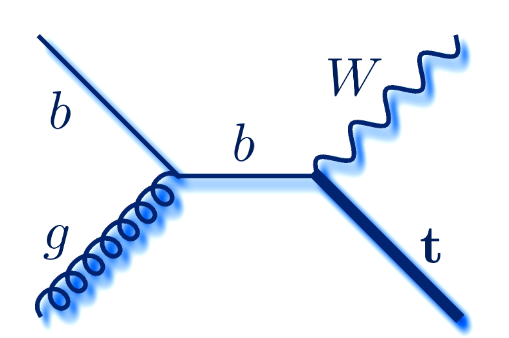
\includegraphics[width=.3\textwidth]{Chapter3/Wt-channel.png}}\hfill
	\subfloat[s-channel]{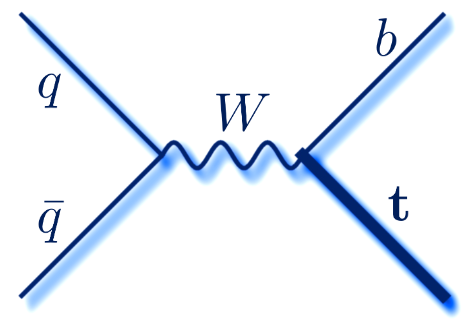
\includegraphics[width=.3\textwidth]{Chapter3/s-channel.png}}
	\caption{The Feynman diagrams of three channels for single top production.}
	\label{Fig:singletop}
\end{figure}

The generation of $WW/WZ$ events are also through \textsc{SHERPA} v2.2.1 for the event production and the hadronisation. 
\\
\\{\bf Signal Simulation}
\\
\\HVT samples are generated via \textsc{MADGRAPH5} interfaced to \textsc{PYTHIA8} with the the resonance mass points ranged from $300GeV$ to $5TeV$ of $100GeV$ spacing. For simplicity, $g_V=1$ and $g_V=3$ are set for model A and model B with ggF and VBF productions respectively.
\\
\\RS graviton events are also simulated through \textsc{MADGRAPH5} and \textsc{PYTHIA8}, and only the ggF production is considered for this signal. Within the simulation, $r_{c}=1$ is set as the default for the simulation, but it is also reweighted in resonance mass distribution at parton level for $r_{c}=0.5$. This is for the comparison with the result from the CMS collaboration. The decay width of this configuration is expected to be $\approx 6\%$. 
\\
\\The decay width and cross section of HVT and RS graviton are summarised in tab. \ref{Tab:xs_decaywidth}:
\begin{table}[htb]
	\caption{The decay width and cross section of HVT and RSG at $800GeV$, $1.6TeV$, and $2.4TeV$ mass points}
	\centering
		\begin{tabular}{|c|ccc|cc|}
          \hline
          \hline
                   & \multicolumn{3}{c|}{ HVT W' and Z' }                                     & \multicolumn{2}{c|}{ RS $G*$}  \\
              $m$  & $\Gamma$ & $\sigma \times BR(Z' \to WW)$ & $\sigma \times BR(W' \to WZ)$ & $\Gamma$ & $\sigma \times BR(G* \to WW)$ \\
            $[TeV]$& $[GeV]$  & $[fb]$                        & $[fb]$                        & $[GeV]$  & $[fb]$      \\
          \hline
               0.8 & 32       & 354                           & 682                           & 46       & 301   \\
               1.6 & 51       & 38.5                          & 79.3                          & 96       & 4.4 \\
               2.4 & 74       & 4.87                          & 10.6                          & 148      & 0.28 \\
          \hline
         \end{tabular}
	\label{Tab:xs_decaywidth}
\end{table}
\noindent
For NWA Higgs boson, its interference with SM Higgs boson ($125GeV$) is assumed to be negligible as discussed in \ref{sec:signal_intro}. Its narrow decay width is set as a constant at $4.07MeV$ over all mass points beyond experimental resolution from the production of ggF and VBF, which are simulated separately. The simulation is done by \textsc{Powheg-Box} v2 showered with \textsc{PYTHIA8} under \textsc{CTEQ6L1} PDF set. 
\\
\\{\bf Derivation}
\\
\\To boost the power of the computational system, the analyses are not operated on AODs directly, but they will be going through the `` derivation'' procedure composed of ``trimming'' and ``slimming'' to drop down variables and events of no interest first, and the outcome data format is called derived AOD (DAOD). For the broad variety of analysis types, a couple of derivation schemes are applied, and the analyese with similar final state share the same derivation scheme. 
\\
\\With the final state of this analysis, ``HIGG5D2'' is chosen with the derivation scheme as the following:
\begin{itemize}
  \item trigger: passing at least one electron, muon, or $E^{T}_{missing}$ trigger
  \item lepton: one electron or muon with $p_{T}>15GeV$ 
  \item jet: two small R jets with $p_{T}>20GeV$, one  small R jet with $p_{T}>100GeV$, or one large R jet with $p_{T}>150GeV$
\end{itemize}
\section{Physical Object Definition}
Because LHC is using protons as the beam source, it leads to enormous production of hadronic jets. Within the environment, most of objects except for jets have great containmination from jet misidentification into other objects. Therefore, the object definitionn for this anlysis is to keep the signal efficiency and the purity of the intended objects at the same time. 
\\
\\{\bf Electron}
\\
\\The electrons in this analysis are defined as two types, loose and signal, to exactly select one signal lepton with no additional loose one. Signal electrons are required to have $p_{T}$ above $27GeV$ to reach the trigger efficiency turn-on plateau, and $|\eta|<2.47$ is applied on both electrons within the acceptance of inner detector while with the crate region vetoed. The impact parameter requirement is set to only consider the electrons from the primary vertex. The full selection criteria is shown in Tab. \ref{Tab:eledefin}.
\\
\\In addition to the fundamental quality requirement, the overlap removal is applied afterwards to prevent the objects reconstructed from the same detector signature. When a electron shares inner detector tracks with muon candidates, the electrons is discarded. The existence of a nearby jet defined as $0.2<\Delta R(e,j)<min(0.4,0.04+10/p_{T}(e)[GeV])$ also makes the electron dropped down. The final requirement on electron is that it shall be consistent with the trigger level electron which fired the required electron trigger to suppress the QCD background. 
\begin{table}[htb]
	\caption{Selection for electron candidates used in the analysis. Veto and signal electrons are defined.}\label{Tab:eledefin}
	\centering
	\begin{tabular}{|c||c|c|}
		\hline
		& \multicolumn{2}{c|}{ Electrons}\\
		&   Loose & Signal \\
		\hline
		$p_T$ & $>7GeV$ & $>27GeV$  \\
		\hline
		$| \eta |$ &  \multicolumn{2}{c|}{ $< 2.47 ~ \notin [1.37,1.52]$ } \\
		\hline
		Identification & LooseLH & TightLH   \\
		\hline
		Isolation       &   LooseTrackOnly & FixedCutTight  \\
		\hline
		$|d_0/\sigma(d_0)^{BL}|$ &   \multicolumn{2}{|c|}{  < 5}  \\
		\hline
		$|z_0\sin\theta| $  & \multicolumn{2}{|c|}{< 0.5~mm}  \\
		\hline
	\end{tabular}
\end{table}
\noindent
\\{\bf Muon}
\\
\\Similar to electrons, loose and signal muons are defined with $p_{T}$ and $|\eta|$ cuts in the consideration of trigger turn-on curve plateau and inner detector coverage. The requirement on muon impact parameters is tightened for better rejection to the cosmic muons. The selection criteria is shown below in Tab. \ref{Tab:mudefin}
\\
\\As muons have the lowest misidentification rate, they are kept in most cases for overlap removal. The only exception is the muons decayed from heavy flavour quark. To remove this type of contamination, the muons are discarded under the scenarios:
\begin{itemize}
	\item $\Delta R(\mu,j)<0.2$
	\item $\Delta R(\mu,j)<min(0.4,0.04+10/p_{T}(\mu)[GeV])$ with the jets fulfilling either of the conditions: a) $p_{T}^{\mu}/p_{T}^j<0.5$ and number of jet-associated tracks greater than 2, b) $p_{T}^{\mu}/\sum^{n}_{1} p_{T}^{trk}<0.7$ for all the jet-associated tracks and $n>2$.
\end{itemize}
This is to reject the muons from heavy flavour quark decay. The last selection in muon is that it shall be spatially consistent to the trigger muon if muon trigger is fired in the event. 
\begin{table}[htb]
	\caption{Selection for muon candidates used in the analysis. Veto and signal electrons are defined.}\label{Tab:mudefin}
	\centering
	\begin{tabular}{|c||c|c|}
   \hline
& \multicolumn{2}{c|}{Muons}\\
\cline{2-3}
&  Loose & Signal  \\
\hline
$p_T$ threshold &  7~GeV & 27~GeV  \\
\hline
$| \eta |$      &  $< 2.7$ & $< 2.5$   \\
\hline
Identification  &  Loose & Medium  \\
\hline
%Track Quality   &  - & - & ''Loose Muon'' & ''Loose Muon'' \\
Isolation       &   LooseTrackOnly & FixedCutTightTrackOnly  \\
\hline
$|d_0/\sigma(d_0)| w.r.t. BL$ &   \multicolumn{2}{|c|}{< 3} \\
\hline
$|z_0\sin\theta| $ &   \multicolumn{2}{|c|}{< 0.5~mm} \\
\hline
	\end{tabular}
\end{table}
\noindent
\\{\bf Small R Jets [R=0.4]}
\\
\\In the intended final states, the jets (denoted as $j$) come from the decay of W bosons ($W\to jj$) or the remnant quarks from vector boson fusion ($jj\to WWjj$ or $jj \to WZjj$). Because of the different kinematic properties, the two types of jets are selected respectively (detail of the pair selection is in Sec. ). The full selection criteria are in Tab. \ref{tab:sjdefinit}.
\\
\\The pair of VBF jets are supposed to be energetic with wide separation, so they have tighter $p_{T}$ selection of $p_{T}>30GeV$ but looser $|\eta|$ cut, $|\eta|<4.5$. For signal jets, they are only required to have $p_{T}>20GeV$, and only the ones with the acceptance of inner detector ($|\eta|<2.5$) are taken as jet candidates for event selection. The jet quality requirement is to remove the ``fake jets'' from calorimeter noise pulse, cosmic ray, or non-collision background (like beam-halo), which is ``called jet cleaning''.

\begin{table}[tbh]
	\caption{Selection for small-R jets}\label{tab:sjdefinit}
	\vspace{2.0em}
	\centering
	\begin{tabular}{|c||c|c|}
		\hline
		             & \multicolumn{2}{|c|}{ Small-R Jets }\\
		\hline
		             & Signal Jets & VBF Jets \\
		\hline
		Algorithm    & \multicolumn{2}{|c|}{ anti$-k_t$, $R=0.4$}\\
		\hline
		$p_T$        & $>20GeV$ & $>30GeV$\\
		\hline
		|$\eta$|     & $< 2.5$ & $<4.5$  \\
		\hline
		Quality      & \multicolumn{2}{|c|}{not ``bad'' jet}\\
		\hline
		JVT          & \multicolumn{2}{|c|}{$< 0.59$ ( $| \eta | < 2.4 ~ \& \& ~p_T < 60 $ GeV)} \\
		\hline
		b-Tagging    & \multicolumn{2}{|c|}{\texttt{MV2c10}, 85\% efficiency} \\
		\hline
	\end{tabular}
\end{table}
\noindent
{\bf Large R Jets [R=1.0]}
\\
\\When the W or Z boson is highly boosted, the two decayed quarks could not be resolved into small R jets, so the large R jets (or called ``fat jets'' and denoted as $J$) are reconstructed to collect the energy deposit. The full selection on the fat jets could be seen in Tab. \ref{Tab:Jdefinit}. However, the jet mass and $p_{T}$ are evaluated with further correction from track-assisted mass, $m^{TA}$, due to the poor spatial resolution in calorimeter. $m^{TA}$ is evaluated to from the tracks left by charged jet partons defined as:
\begin{equation}
m^{TA} = m^{trk} \times \frac{p_{T}^{J}}{\sum p_{T}^{trk}}
\end{equation}  
Here, $m^{trk}$ is the reconstructed mass of the tracks taken as massless particles, and $p_{T}^{trk}$ is the vector sum from $p_{T}$ of tracks.  The ratio of $p_{T}$ between tracks and the jet is to take in the neutral-to-charge fluctuations. It could then be combined with calorimeter mass, $m^{calo}$, into combined mass, $m^{comb}$, by the definition:
\begin{equation}
m^{comb} = \frac{\sigma_{{calo}}^{-2} m^{{calo}} + \sigma_{{TA}}^{-2} m^{{TA}} }{\sigma_{{calo}}^{-2} + \sigma_{{TA}}^{-2}}
\end{equation}
with $\sigma_{{calo}}^{-2}$ and $\sigma_{{TA}}^{-2}$ as pre-estimated mass resolution for calorimeter and track-assisted mass which are assumed to be uncorrelated. From Fig. \ref{Fig:combinedmassperformance}, it could be seen that calorimeter mass has better performance in the low $p_{T}(W)$ regime benefited from the great energy resolution, but it is degraded in high $p_{T}(W)$, and track-assisted mass performed in an opposite way. The combined mass takes the merits of the two mass definitions and provide the best mass resolution ($\tilde 10\% (15\%)$ at jet $p_{T}=1TeV(2.5TeV)$) , so it is taken as the nominal mass in this analysis with the selection of $m^{comb}>50GeV$. The correction on $p_{T}$ is then performed as $p_{T}^{comb}=p_{T}^{calo}\times m^{comb}/m^{calo}$ 

\begin{table}[h]
	\caption{Selection for large-R jets}\label{Tab:Jdefinit}
	\vspace{2.0em}
	\centering
	\begin{tabular}{|c||c|}
		\hline
		& Signal Large-R Jets\\
		\hline
		Algorithm & anti$-k_t$, $R=1.0$\\
		$p_{T}$   & >200~GeV\\
		$| \eta |$      & $< 2.0 $\\
		Mass threshold  & 50~GeV\\
		W/Z Tagger &  $D^{\beta =1}_2 \& m^{comb}$ \\
		\hline
	\end{tabular}
\end{table}
\begin{figure}[ht]
	\begin{center}
		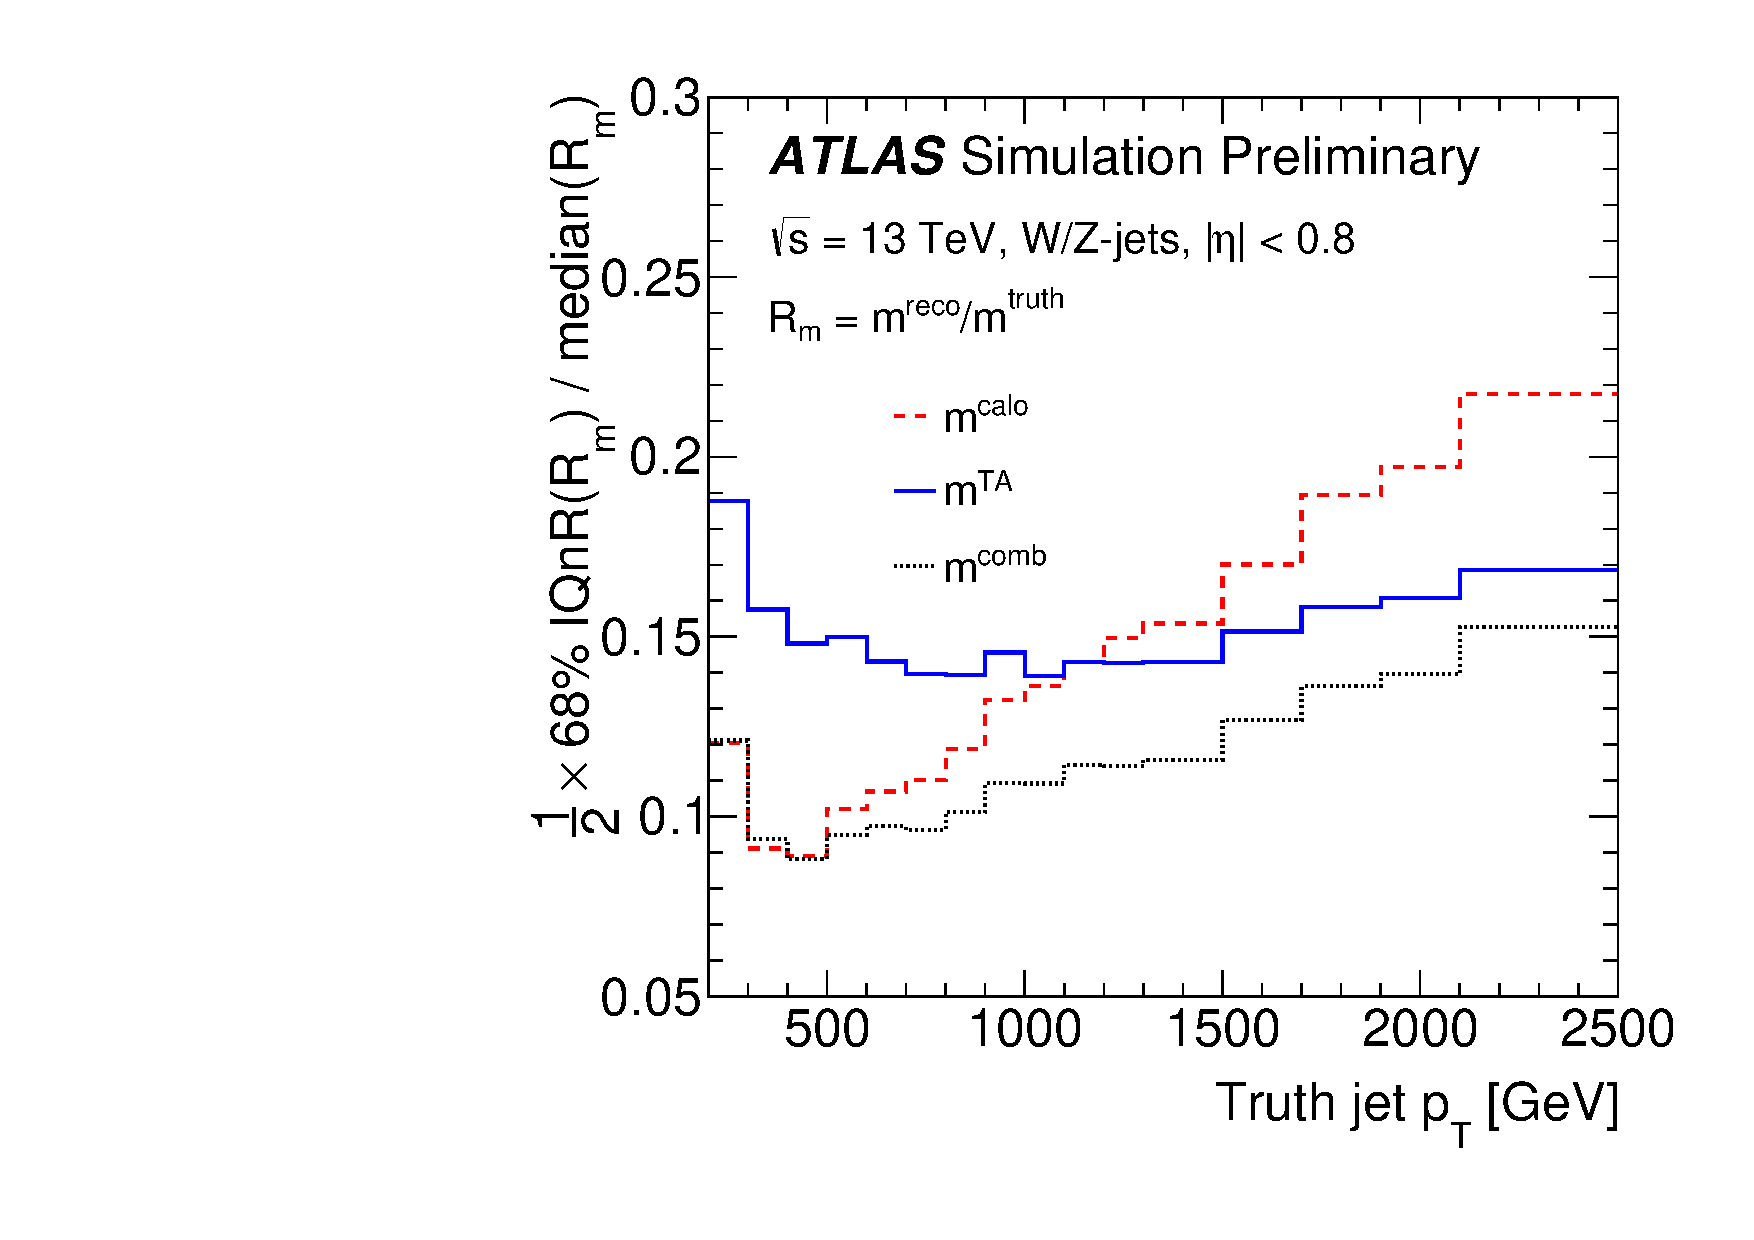
\includegraphics[width=0.6\hsize]{Chapter3/mass_resolution}
		\caption{The jet mass resolution as a function of jet $\p_{T}$ for jets produced from boosted $W$ boson\cite{ATLAS-CONF-2016-035}. Three different jet mass reconstruction algorithms are displayed: the calo-jet mass ($m^{{calo}}$), the track-assisted mass ($m^{{TA}}$), and the combined TA+calo mass ($m^{{comb}}$).}
		\label{Fig:combinedmassperformance}
	\end{center}
\end{figure}
\noindent
However, the combined mass is still not proficient to select the W/Z decayed fat jets precisely, so the substructure of jets is needed to improved the boson tagging. It is patterned by  $R=0.2$ subjets from $k_{T}$ algorithm on the topoclusters, and only the ones meeting the condition, $p_{T}^(subjet)/p_{T}^{R=1.0}>0.05$, are kept and ``ghost-associated'' to the fat jets. The correlation between the subjets could then give the discriminant, $D^{\beta =1}_{2}$, for W/Z boson recognition:
\begin{equation}
D^{\beta =1}_{2} = \frac{e^{\beta}_{3}}{e^{\beta}_2} 
\end{equation}
with $e^{\beta}_{2}$ and $e^{\beta}_{3}$ as:
\begin{equation}
e^{\beta}_{2} = \frac{1}{(p_{T}^{jet})^2}\displaystyle\sum\limits_{i<j\in J}p_{T}^{i}p_{T}^j(R_{ij})^{\beta}
\end{equation}
\begin{equation}
e^{\beta}_{3} = \frac{1}{(p_{T}^{jet})^3}\displaystyle\sum\limits_{i<j<k\in J}p_{T}^{i}p_{T}^{j}p_{T}^{k}(R_{ij}R_{jk}R_{ik})^{\beta}
\end{equation}
where i, j, and k are the index for the subjets. The boson tagging is then done by a 2D cut on both $D^{\beta =1}_{2}$ and $m^{comb}$ as a function of $p_{T}$ shown in Fig. \ref{Fig:newWZtaggerWP}. Two working points are used in this analysis: $50\%$ and $80\%$. 
\begin{figure}[ht]
	\begin{center}
		\subfloat[]{
			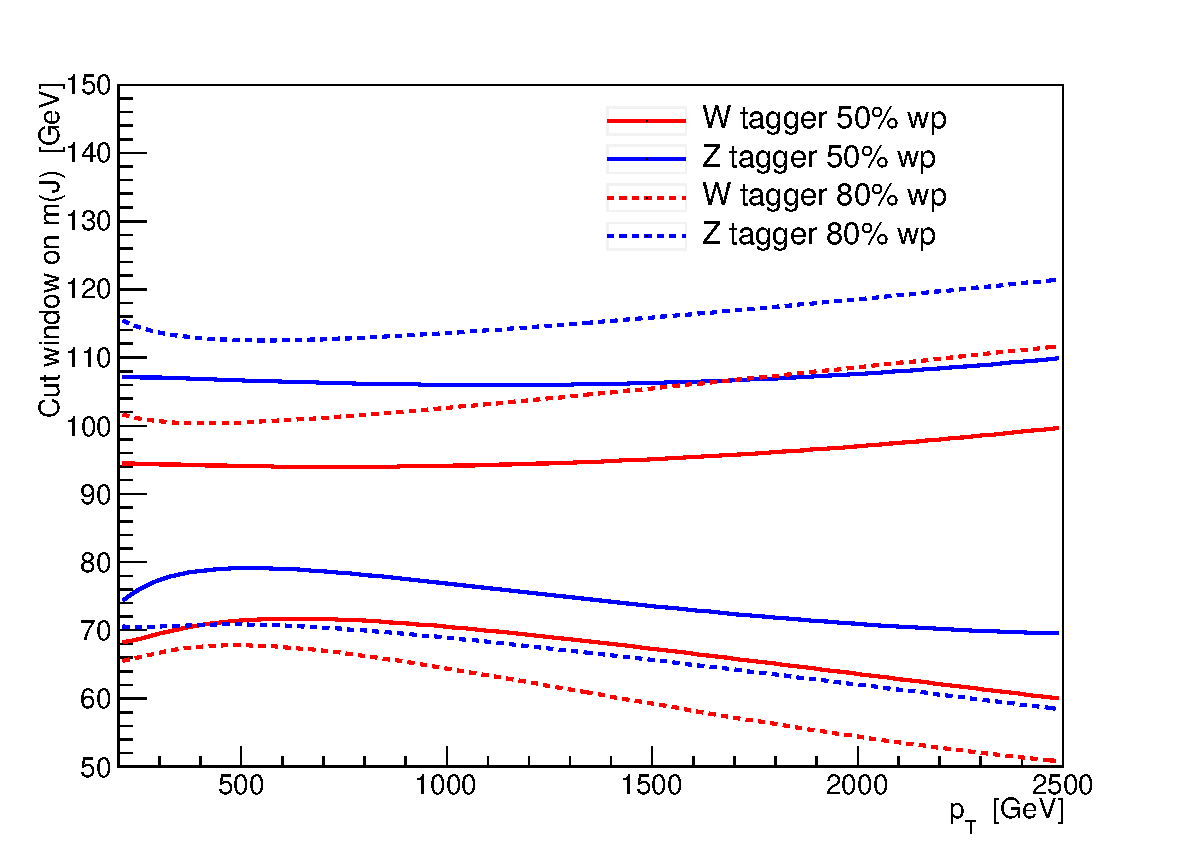
\includegraphics[width=0.48\hsize]{Chapter3/MassWindow_newWZTagger}
		}
		\subfloat[]{
			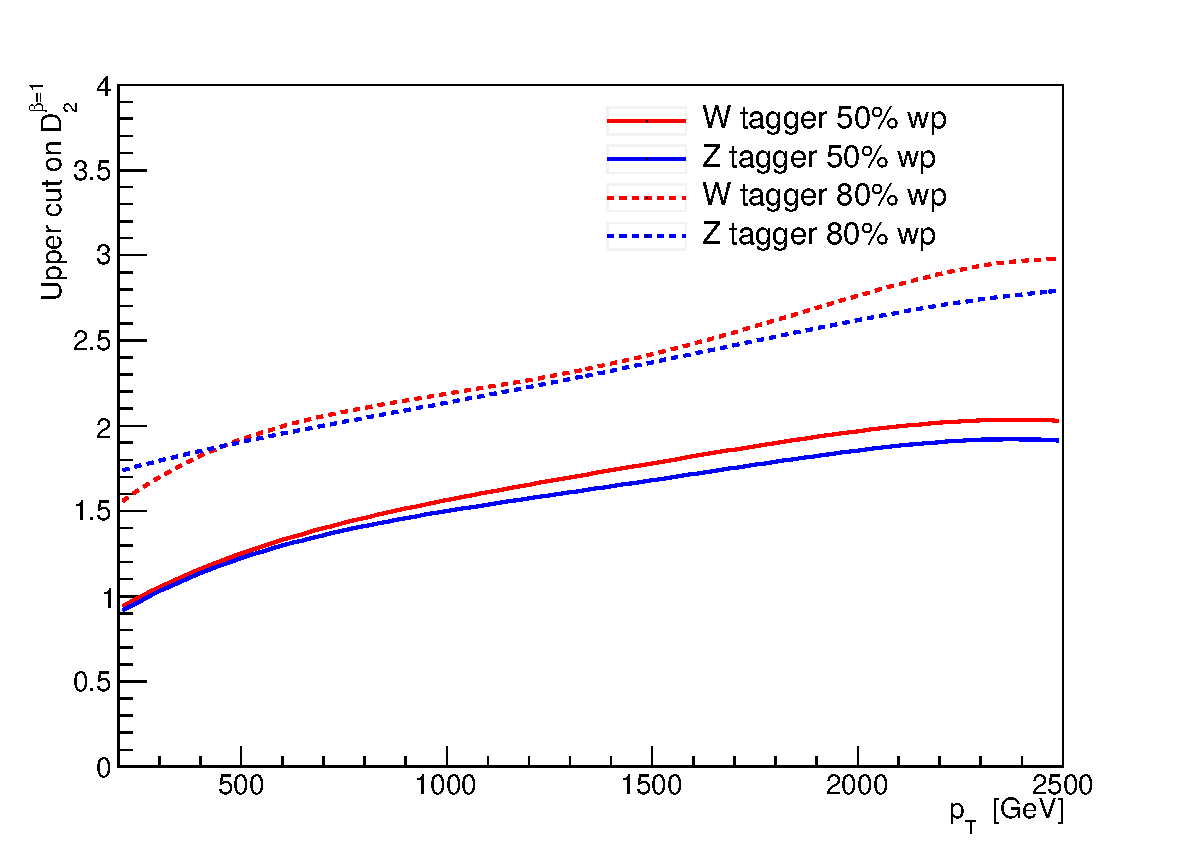
\includegraphics[width=0.48\hsize]{Chapter3/D2UpperCut_newWZTagger}
		}
		\caption{The thresholds of the mass window cut (a) and the upper cut on $D^{\beta =1}_2$ (b) as a function of $p_{T}$ used in this analysis. The cuts  for $W$-($Z$)-boson tagging is shown by red (blue) lines.}
		\label{Fig:newWZtaggerWP}
	\end{center}
\end{figure}
\noindent
{\bf Missing Transverse Energy}
\\
\\Although $E^{missing}_{T}$ is supposed to be reconstructed as how Sec. \ref{sec:obj rec} describes, tau and photons are treated as jets for the intended final state. The cut on $E^{miss}_{T}$ will be discuss in next section.   
\section{Event Selection}
The event selection is conducted to maximize the sensitivity by removing background events but also keep the signal at the same time. To achieve this purpose, the significance is defined as:
\begin{equation}
\label{Eq:significance}
\sigma_{sig} = \displaystyle\sum_{i}^{N_{bin}}( \frac{s_i}{s_i+b_i+(\Delta_bi)^2})^2
\end{equation}
where $s_i$ and $b_i$ are the signal and background event numbers in each bin on $m_{WV}$ distribution. The cuts on the variables would be varied on signal and background samples simultaneously, and the final criteria is given by the combination of cuts with the best significance. The signal sample applied in the optimization could be either via the medium state of WW or WZ, as they have similar kinematic properties. However, they are still divided into two subchannels with the definition of dedicated mass windows.  
\\
\\Then, the events in this analysis are further categorized by jet topologies, VBF jets selection and fat jet recognition into different regions prioritized by the signal sensitivity. In general, the VBF production events could gain better sensitivity than the ggF/DY production ones, and the events with fat jets which are called ``boosted'' events are also more sensitive than the ones with only small R jets, so they are granted with higher priority. Fig. \ref{Fig:order} shows how the events are categorized by the given priority. For the events which fail part of the jet selection, they would go into the control regions to constrain the background contribution from W+jets and $t\bar{t}$ which are the two dominant backgrounds in this analysis. The two control regions are used in the simultaneous fitting to derive the scale factor of background estimation, and the details will be discussed in next chapter
\begin{figure}[h]
	\centering
	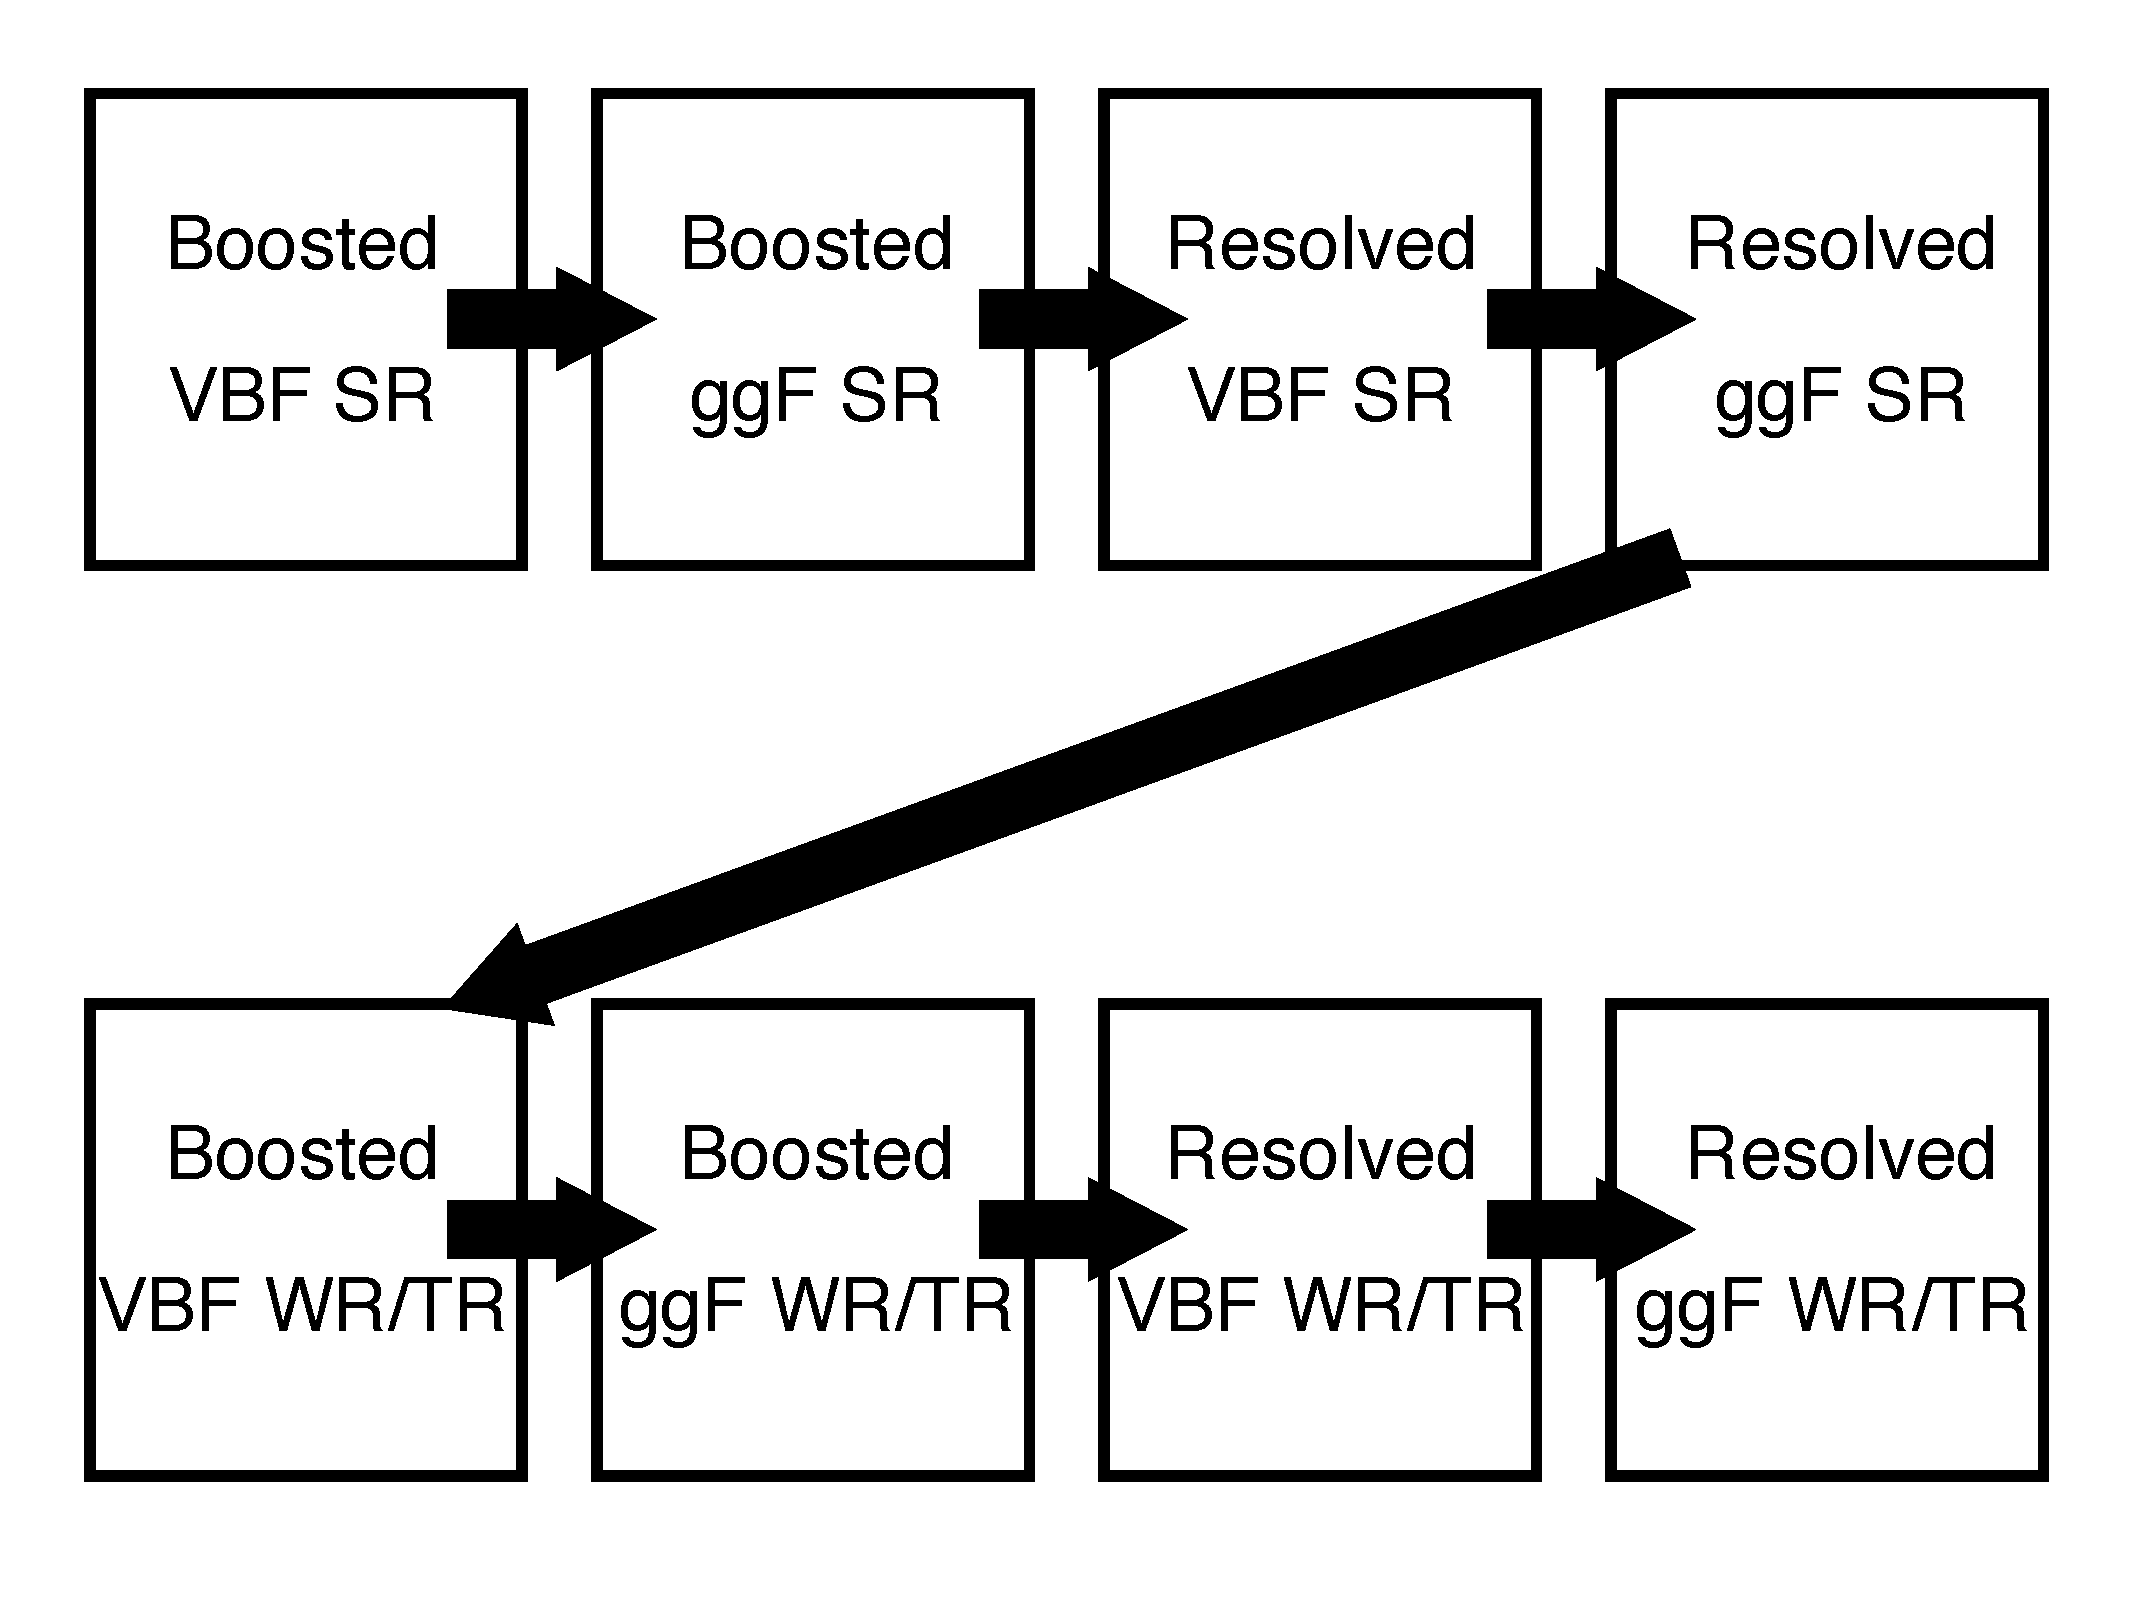
\includegraphics[width=0.7\hsize]{Chapter3/order}
	\caption{Illustration of how to combine the SR/CRs in this analysis.}
	\label{Fig:order}
\end{figure}

\subsection{Trigger}
\label{Subsec:Trigger_resonance}
The first applied criterion on event selection is trigger. The recorded data is a broad collection of different physical signatures, and the final state in the analysis only accounts for a small fraction of them. Therefore, certain triggers which could be fired by the signatures from our final state is required, which are the electron, muon, and $E^{miss}_{T}$ triggers. Because of the increasing luminosity provided by LHC, the trigger threshold was enhanced in 2016 to reduce the trigger rate. For the MC samples, run number is randomly generated, and the events shall only pass the triggers available in the random run number. The full trigger set used in this analysis is shown in Tab. \ref{tab:triggers}
\begin{table}[h]
	\caption{The list of triggers used in the analysis.} \label{tab:triggers}
	
		\footnotesize
		\begin{center}
		\begin{adjustbox}{center}
			\begin{tabular}{|l|c|c|c|}
				\hline
				\multirow{2}{*}{Data-taking period} & \multirow{2}{*}{Electron channel} & \multicolumn{2}{c|}{ Muon channel }  \\
				\cline{3-4}
				& & $p_{T},\left(\mu\nu\right) < 150\,GeV$ & $P_{T},\left(\mu\nu\right) > 150\,GeV$   \\
				\hline
				\multirow{3}{*}{\centering {2015}} & HLT\_e24\_lhmedium\_L1EM20 & HLT\_mu20\_iloose\_L1MU15 & \multirow{3}{*}{ HLT\_xe70 } \\
				& HLT\_e60\_lhmedium  & HLT\_mu50 & \\
				& HLT\_e120\_lhloose & & \\
				\hline
				\multirow{2}{*}{\centering {2016a (run $< 302919$)}} & HLT\_e26\_lhtight\_nod0\_ivarloose & HLT\_mu26\_ivarmedium  & \multirow{3}{*}{ HLT\_xe90\_mht\_L1XE50 } \\
				& HLT\_e60\_lhmedium\_nod0 & HLT\_mu50 &  \\
				($L<1.0\times10^{34}\,{ cm}^{-2}\,{s}^{-1}$) & HLT\_e140\_lhloose\_nod0 & & \\
				\hline
				{\centering {2016b (run $\geq 302919$)}} & \multirow{2}{*}{same as above} & \multirow{2}{*}{same as above}  &  \multirow{2}{*}{HLT\_xe110\_mht\_L1XE50} \\
				($L<1.7\times10^{34}\,{ cm}^{-2}\,{ s}^{-1}$) & & &\\
				\hline
				\hline
				Total int. lumi. [$fb^{-1}$] &  36.1 & 35.6 & 35.9 \\
				\hline
			\end{tabular}
		\end{adjustbox}
		\end{center}
	
\end{table}
\noindent
Three electron triggers are used in electron channel including the unprescaled lowest threshold one to maximize the signal efficiency. The other two triggers are used to select high $\p_{T}$ electrons with looser isolation requirement. The combined performance of the triggers is around $90\%$ efficiency at the turn-on plateau as a function of $p_{T}$.
\\
\\In muon channel, both $E_{T}^{miss}$ and muon triggers are used. For the scenario of $p_{T}(\mu\nu)<150GeV$, the unprescaled lowest threshold muon trigger is used accompanied by the higher threshold one without isolation requirement. Otherwise, $E^{T}_{miss}$ trigger is chosen for $p_{T}(\mu\nu)>150GeV$ events. The reason for this trigger combination is that muon trigger can only reach $70\%$ efficiency on the plateau, so $E^{miss}_{T}$ trigger is added to compensate the lost efficiency. 
\\
\\However, the $E^{miss}_{T}$ cut in this analysis is below the plateau, so there might be the inconsistency between data and simulation in terms of efficiency. Therefore, ``tag and probe'' method is applied to study the trigger efficiency as a function of $p_{T}(\mu\nu)$ (because muons are invisible in trigger level, trigger level $E_{T}^{miss}$ is actually $p_{T}(\mu\nu)$). This study is performed on boosted and resolved channel respectively. The tagged events are required to fulfil the following conditions for resolved (boosted) channel: a) one muon with $p_{T}>27GeV$ b) $E^{miss}_{T}>60(100)GeV$ c) at least 2 signal jets (1 fat jet) selected d) the unprescaled lowest threshold muon trigger is fired. The events are then probed by whether $E^{miss}_{T}$ trigger is fired to give the efficiency. The result for data and simulated $t\bar{t}$ events are shown in Fig. \ref{Fig:eff_met_merged} for boosted channel  in Fig. \ref{Fig:eff_met_resolved} for resolved channel. The efficiency reaches the plateau at $200GeV$, but $E^{miss}_{T}$ trigger is applied for $p_{T}(\mu\nu)>150GeV$, so the scaling factor is taken into simulation as the extra event weight to make them consistent. 
\begin{figure}[ht]
	\begin{center}
		\subfloat[]{
			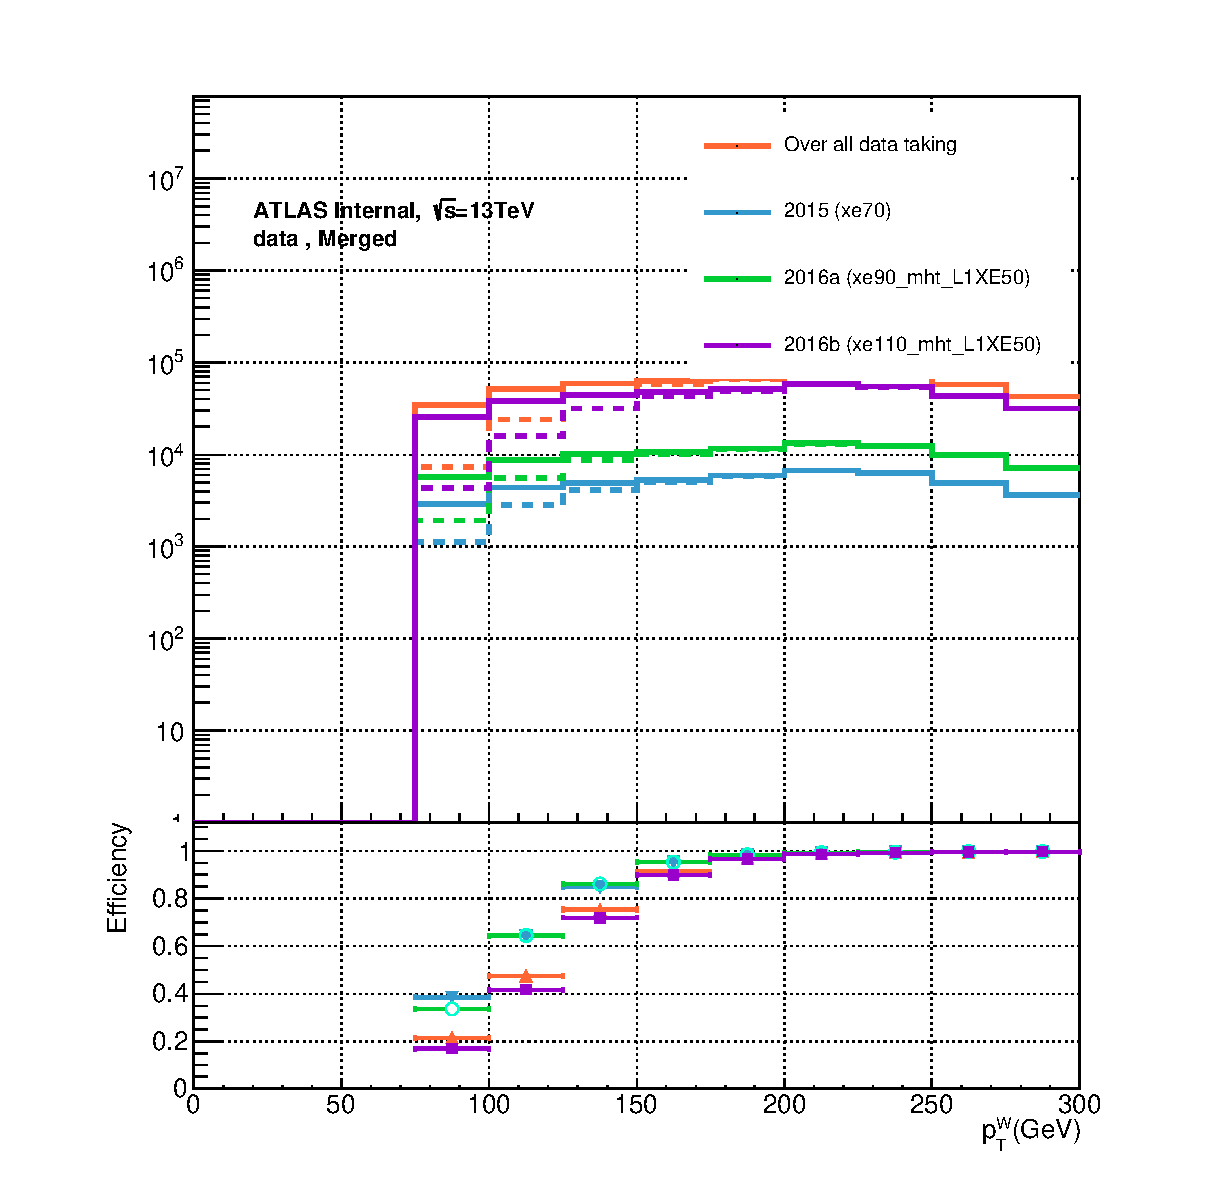
\includegraphics[width=0.48\hsize]{Chapter3/Merged_TrigEff_ptW_METcut_data.eps}
		}
		\subfloat[]{
			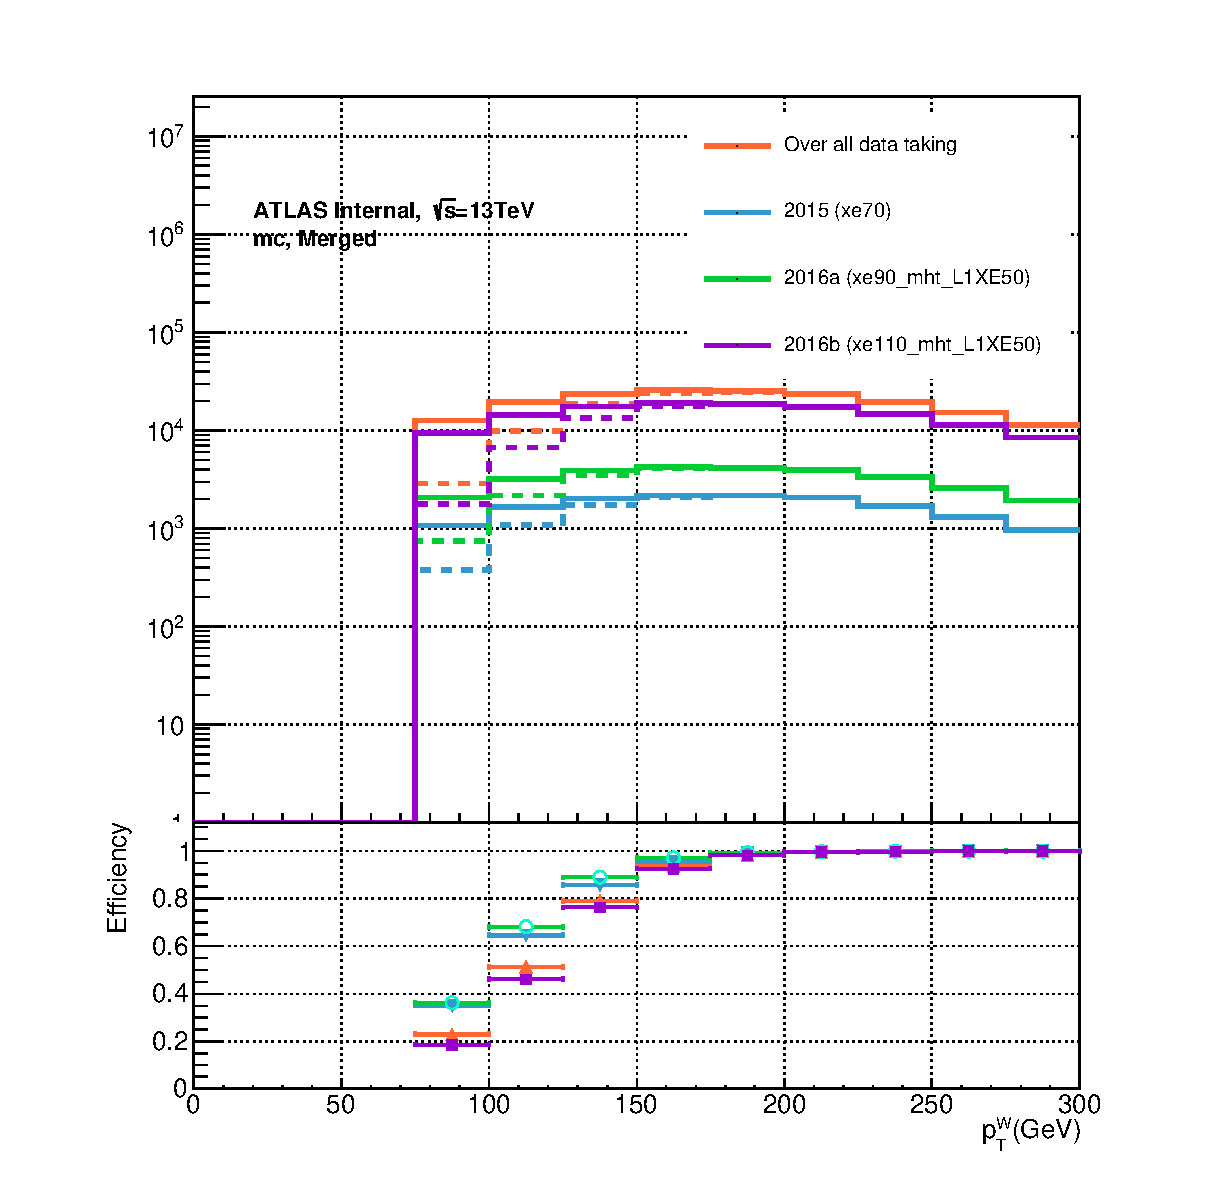
\includegraphics[width=0.48\hsize]{Chapter3/Merged_TrigEff_ptW_METcut_ttbar.eps}
		}
		\caption{The upper plot is $p_{T}(\mu\nu)$ distribution of tagged (real) and probed events in boosted channel for data (a) and $t\bar{t}$ events (b). The lower plots is the efficiency as a function of $p_{T}(\mu\nu)$}
		\label{Fig:eff_met_merged}
	\end{center}
\end{figure}

\begin{figure}[ht]
	\begin{center}
		\subfloat[]{
			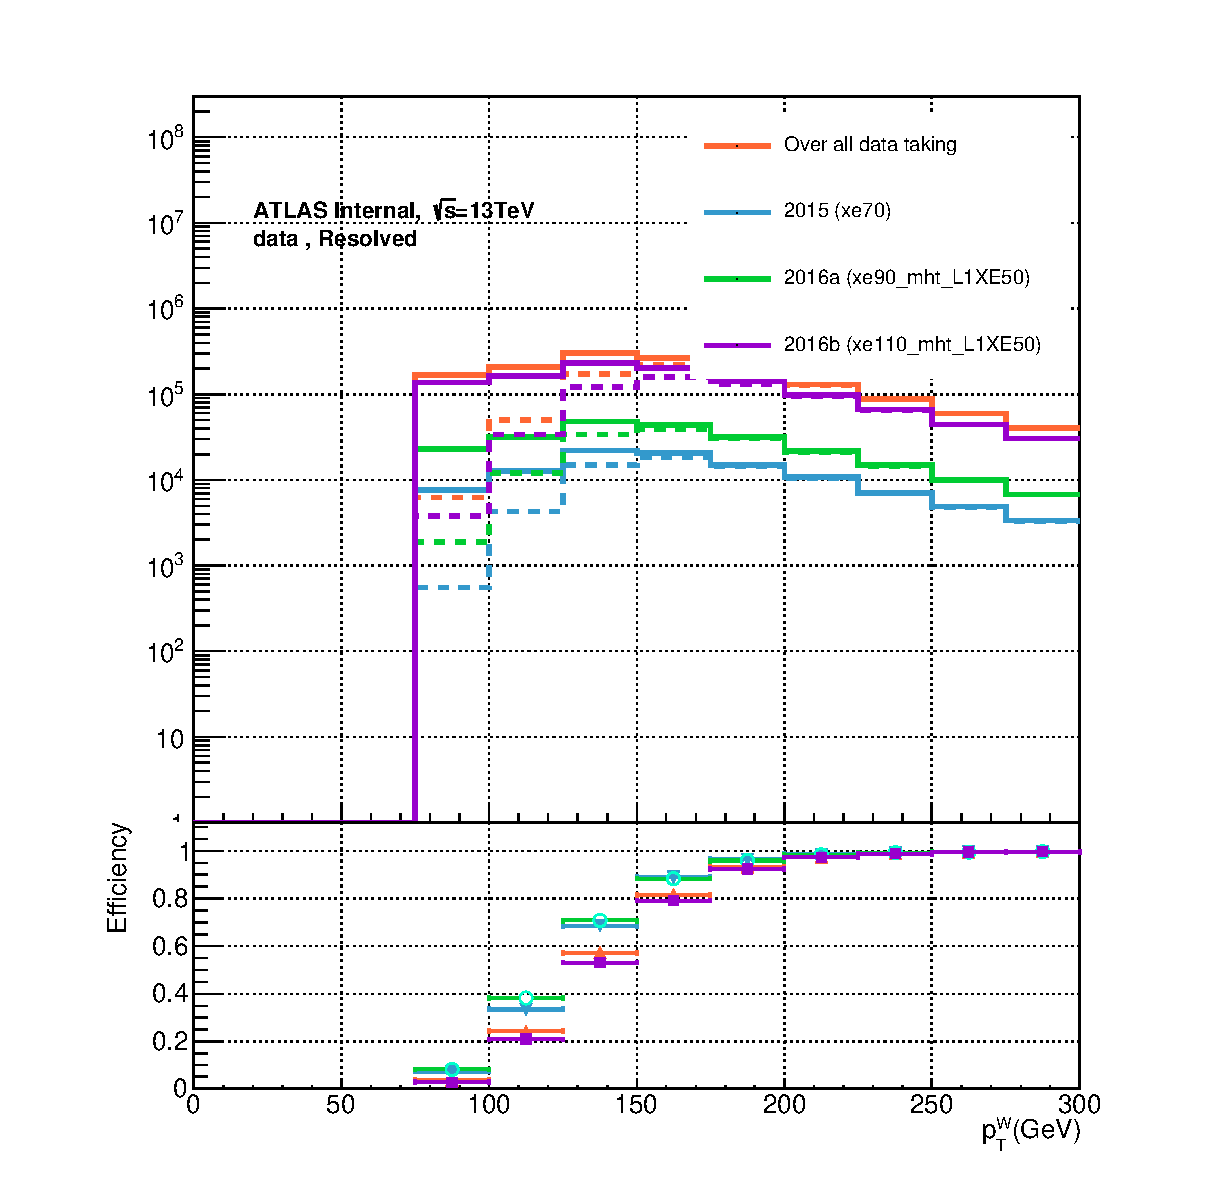
\includegraphics[width=0.4\hsize]{Chapter3/Resolved_TrigEff_ptW_METcut_data.eps}
		}
		\subfloat[]{
			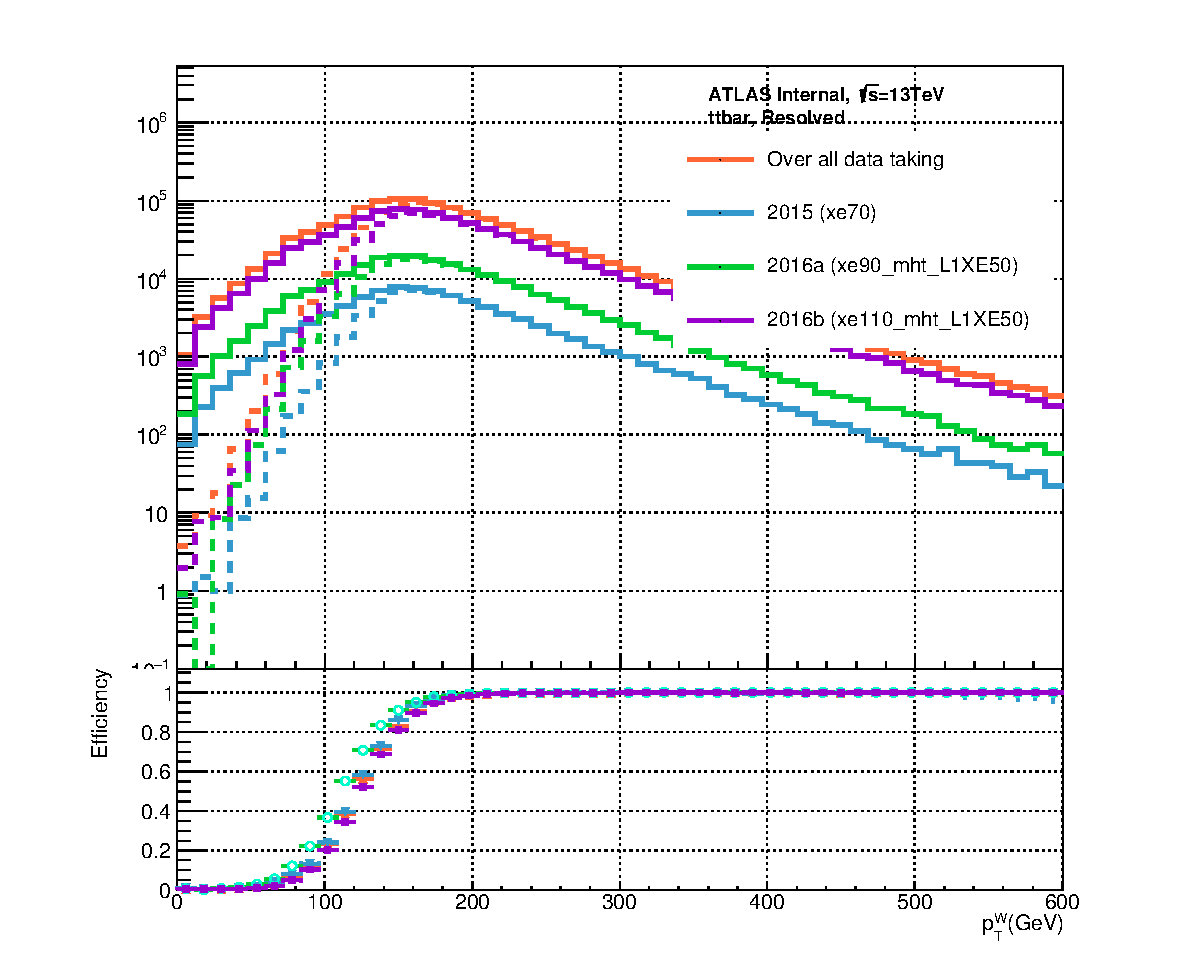
\includegraphics[width=0.48\hsize]{Chapter3/Resolved_TrigEff_ptW_METcut_ttbar-eps-converted-to}
		}
		\caption{The upper plot is $p_{T}(\mu\nu)$ distribution of tagged (real) and probed events in resolved channel for data (a) and $t\bar{t}$ events (b). The lower plots is the efficiency as a function of $p_{T}(\mu\nu)$}
		\label{Fig:eff_met_resolved}
	\end{center}
\end{figure}
\noindent
\subsection{Event Cleaning and Preselection}
After the trigger, the event ``quality is verified by a series of flags in data determining the suitability of an event for physical analysis. The following is the list:
\begin{itemize}
	\item {\bf Good Run}: if the detector operates in a proper status without intolerable defects, they go into the good run list (GRL). Only the events contained in GRL are considered in this analysis. 
	\item {\bf Primary Vertex}: because all the physical objects are required to origin from the primary vertex, its existence is essential. Events without a proper primary vertex (defined in Sec. \ref{sec:obj rec}) are discarded.
	\item {\bf Tile Error Veto}: part of the channels in tile detector are broken. If they accept any physical objects, this flag would be marked, and the events are vetoed.
	\item {\bf LAr Error Veto}: part of the channels in LAr detector are broken. If they accept any physical objects, this flag would be marked, and the events are vetoed.
	\item {\bf SCT Error Veto}: part of the channels in SCT detector are broken. If they accept any physical objects, this flag would be marked, and the events are vetoed.
	\item {\bf Core Error Veto}: during data-taking period, the atlas central DAQ system might suffer from some glitches which broke the data recording, and the flag is marked for events. They are also vetoed in this analysis. 
\end{itemize}
\subsection{Parameter of Interest, $m_{WV}$}
This analysis is searching for the mass resonance of exotic particles, so it is the discriminant to seek for the signal. (i.e. $m_WV$ distribution is the input for statistic interpretation.) However, the longitudinal $p_{T}$ of neutrinos in the final state could not be measured, so the mass resolution is poor to spot the signal spike. Therefore, $p_{z}(\nu)$ is solved with the assumption of $W\rightarrow l\nu$, so the equation of energy conservation could be written down as:
\begin{equation}
m^2_W = m_{l}^{2} + 2E_{l}\sqrt{ p_{T,\nu}^2 + p_{z,\nu}^{2} }  - 2 \vec{p}_{{T},l} \cdot \vec{p}_{T, \nu} - 2 p_{z, l} p_{z,\nu}
\end{equation}
\noindent
In SM, W boson has the mass of $80GeV$, so $m_{l}$ for electron and muon is negligible. This leads to the quadratic equation of $p_{z}^\nu$:
\begin{equation}
4p_{{T}, l}^{2} p_{z,\nu}^{2} - 4 \left( m_{W}^{2} + 2 \vec{p}_{{T}, l} \cdot \vec{p}_{{T},\nu} \right) p_{z,l} p_{z, \nu} - \left( m_{W}^{2} + 2\vec{p}_{{T}, l} \cdot \vec{p}_{{T},\nu}  \right)^{2} +4p_l^{2} p_{{T},\nu}^{2} = 0
\end{equation}
\noindent
If the two outcome solutions are complexes, only the real terms are taken into this analysis. To determine which solution to use, the resolution is compared with absolute value of the two solutions (bigger one and smaller one) defined as:
\begin{equation}
\sigma = \frac{p_z^{truth}-p_z^{\nu}}{p_z^{truth}}
\end{equation}
\noindent
with $p_z^{truth}$ as the neutrino longitudinal momentum at generator level (MC truth). The result could be seen in Fig. \ref{Fig:netrinoPz}, and it indicates the bigger one has slightly better performance, so it is kept.  
\begin{figure}
	\centering
    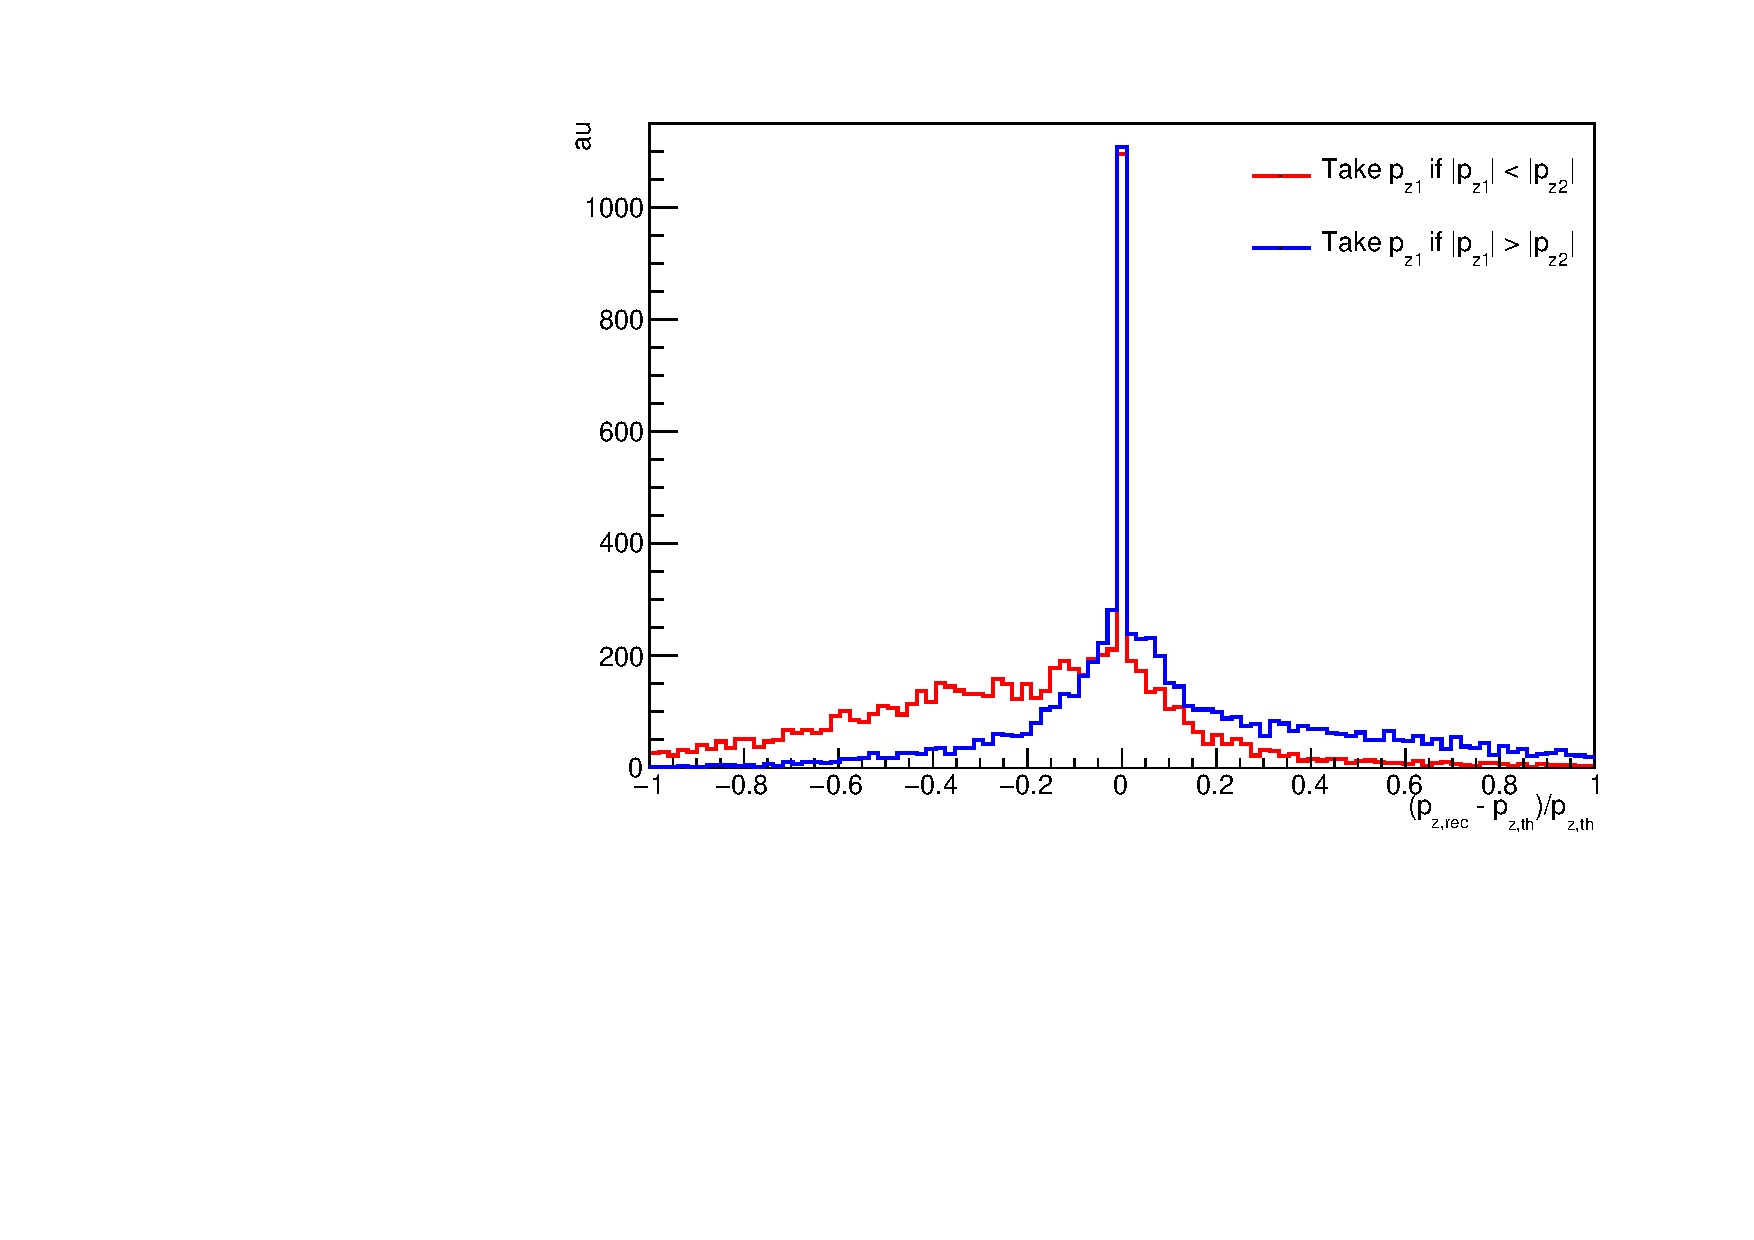
\includegraphics[width=0.5\hsize]{Chapter3/neutrinoPz}
    \caption{The $p_{z}^\nu$ resolution with absolute values of the solutions, bigger and smaller one. }
    \label{Fig:netrinoPz}
\end{figure}
\noindent
In addition to the correction on the leptonically decayed W boson, further improvement on $m_{WV}$ reconstruction is also made by $p_{T}(j,j)$ of the two resolved signal jets by the correction of$p_{T}^{corr}=p_{T}(j,j)\times \frac{m_{V}}{m_{jj}}$ (For WW, $m_V$ is taken as W boson mass, while it is Z boson mass for WZ medium state). The improvement of the ``mass-constraint'' correction could be seen in Fig. \ref{Fig:WHadmassConst} for around $20\%$ better $m_{WV}$ resolution. 
\begin{figure}[h]
	\centering
	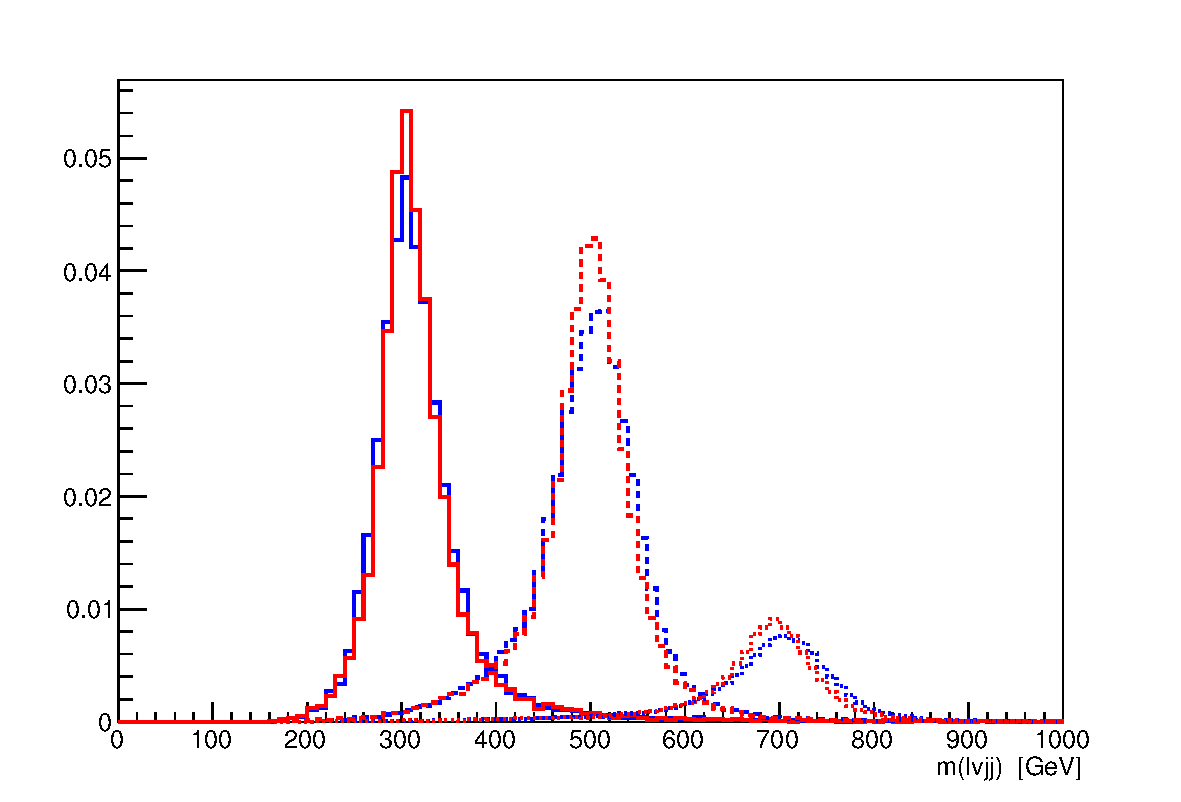
\includegraphics[width=0.6\hsize]{Chapter3/lvjjmass_WmassConstraint}
	\caption{$m_{WV}$ distributions for $gg \rightarrow H \rightarrow WW$ signals at $m=300GeV$ (solid), 500GeV (dashed) and 700GeV (dot), with (red) and without (blue) $W$-mass constraint to $W \rightarrow jj$ system.}\label{Fig:WHadmassConst}
\end{figure}
\noindent
\subsection{VBF Event Selection}
As VBF signal regions have better sensitivity than ggF/DY production, the selection criteria play an important role in this analysis. The optimization on the selection is conducted in three steps. First, all VBF events are required to have at least 4(2) jets in resolved (boosted) channel. Second, the the two jets in the dijet system are supposed to be the pair with the highest mass, opposite $\eta$ signs, and not b-tagged. This pair was chosen prior to the $W/Z\rightarrow jj$ signal jet selection and removed from signal jet candidates. Then, the optimization is performed on a 2-dimensional phase space constructed by $\Delta\eta(j,j)$ and $m(j,j)$ which are two most evident signatures of this production process. The performance of the cuts on the two variables is determined by signal significance in Eq. \ref{Eq:significance}. Fig. \ref{Fig:VBFOptimization} shows the result of the optimization performed on signal with $700GeV$, and the best significance could be achieved by:
\begin{itemize}
	\item {\bf $m_{jj}^{VBF}$}:> 770GeV
	\item {\bf $\Delta\eta(jj)$}: >4.7
\end{itemize}
The other reason to choose this set of cuts is to make it consistent with $WZ/ZZ \rightarrow lljj/\nu\nu jj$ analysis for the combination in next chapter. 
\begin{figure}[h]
	\centering
	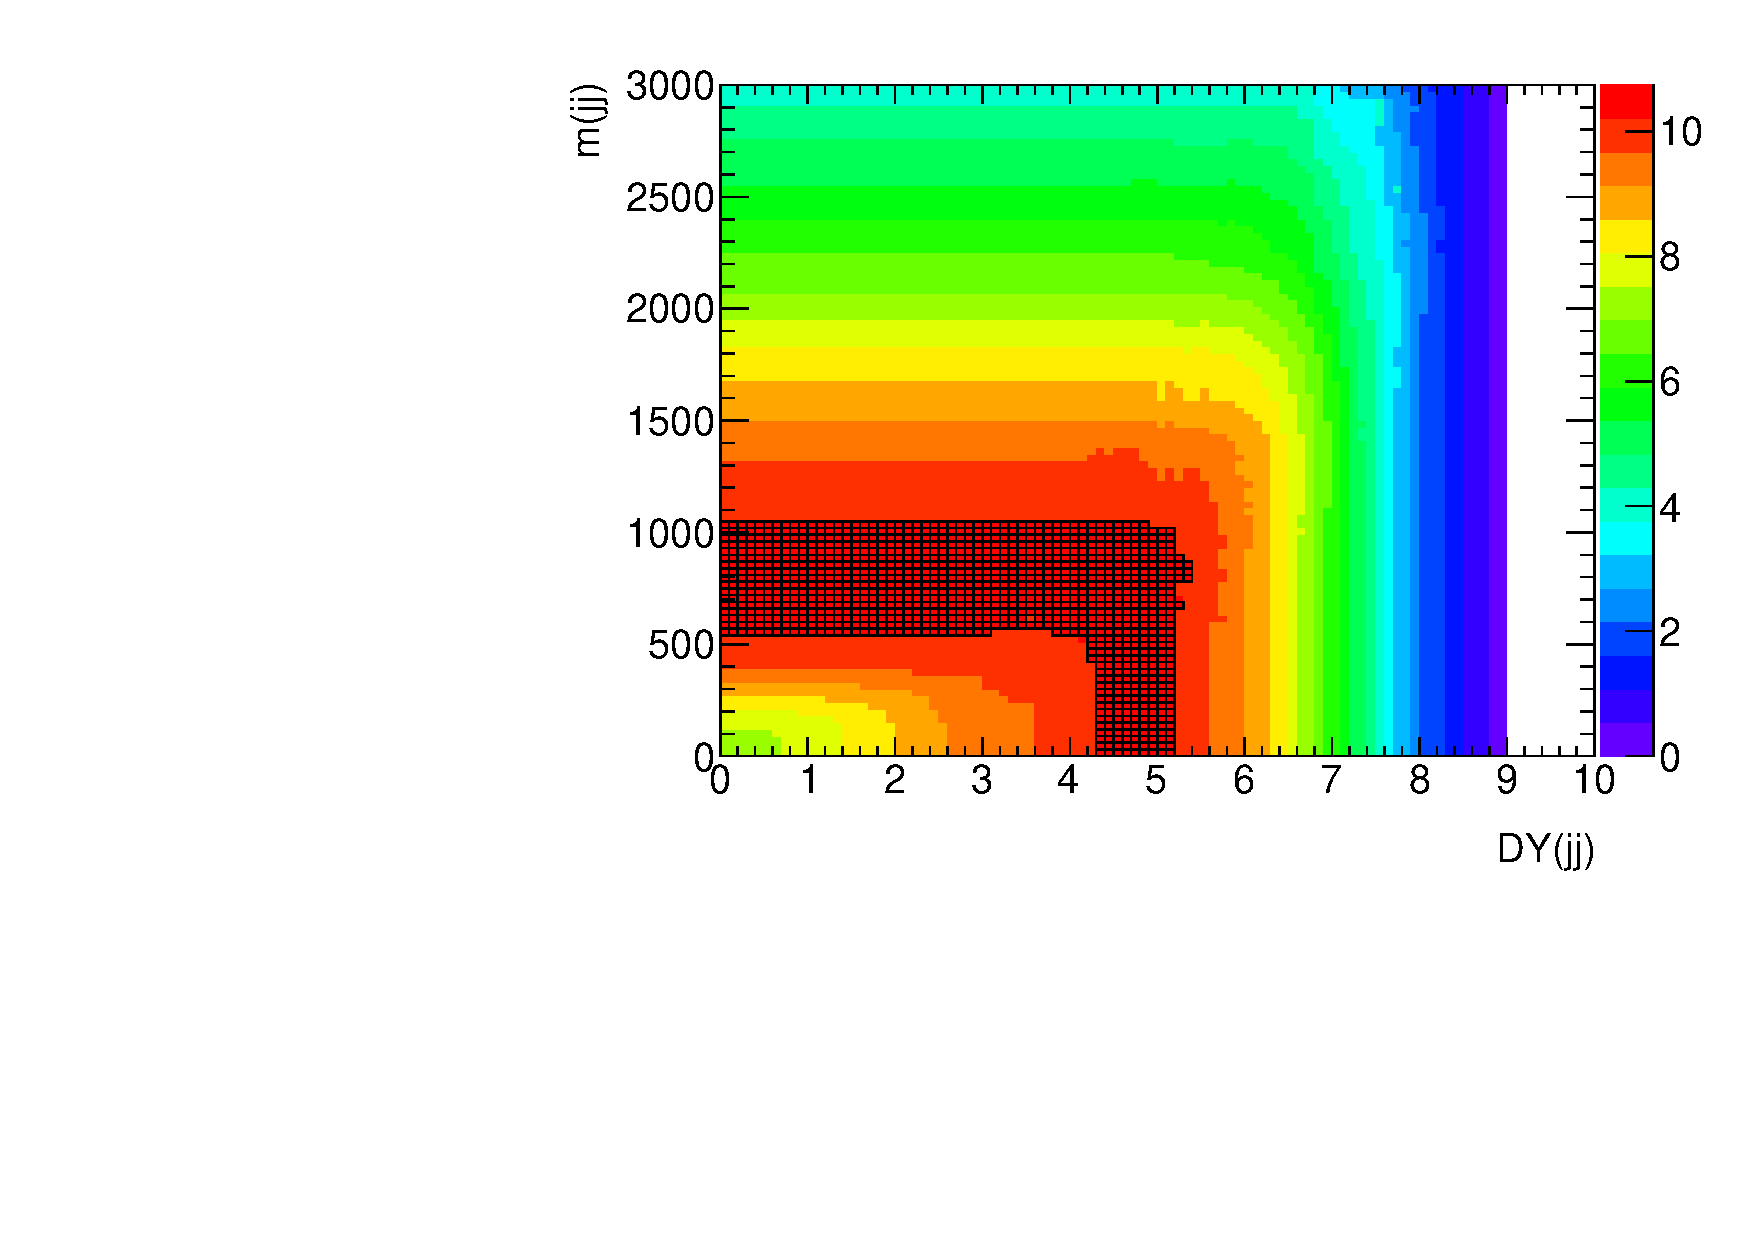
\includegraphics[width=0.7\textwidth]{Chapter3/VBF700_SignfSpace}
	\caption{The signal significance for the VBF $WW$ signal as a function of the VBF cuts $\Delta \eta(j_1,j_2)$ and $m(jj)$ for signal mass 700GeV (right). The black outlined bins are those whose values vary from the maximum by less than 5\%.}
	\label{Fig:VBFOptimization}
\end{figure}
